\documentclass[dvipdfmx,autodetect-engine,10pt,b5paper,papersize,openany,dvipsnames]{jsbook}


\usepackage{color}
\usepackage{titlesec}
\usepackage{multicol}

% 本文をゴシックに
\usepackage[deluxe]{otf}
\renewcommand{\kanjifamilydefault}{\gtdefault}
\renewcommand{\familydefault}{\sfdefault}

\usepackage{amsmath,txfonts}
\usepackage{bm}
\usepackage{mathrsfs} % \mathscr

\usepackage[dvipdfmx]{graphicx}

% PDF を読み込み
\usepackage{pdfpages}

\usepackage{fancyhdr}

\usepackage{tikzpagenodes}
%\usepackage[object=vectorian]{pgfornament}
\usetikzlibrary{shapes.geometric,calc}


% AddToShipoutPictureBG*
\usepackage{eso-pic}


%\usepackage[dvipdfmx]{hyperref}
\usepackage[hidelinks]{hyperref}
\usepackage{pxjahyper}


\usepackage{listings}
\lstset{
  title={},
  caption={},
  frame={single},
  numbers=none,
  lineskip=-0.5ex,
  basicstyle={\small\ttfamily},
  identifierstyle={\small},
  commentstyle={\smallitshape},
  keywordstyle={\small\bfseries},
  ndkeywordstyle={\small},
  stringstyle={\small\ttfamily},
}

% https://oku.edu.mie-u.ac.jp/~okumura/jsclasses/
% jsbook の余白が広すぎます
% 書籍では1行の長さが全角40文字を超えないようにしています。
% そのため,段組をしないときは,自動的にどちらかの余白が広くなります
% (美文書シリーズのようなデザインになります)。
% これが困るときはプリアンブル(\begin{document} の前)に次のように書いてください。
\setlength{\textwidth}{\fullwidth}
\setlength{\evensidemargin}{\oddsidemargin}

%% 上下の余白を20mmにする
\setlength{\textheight}{\paperheight}   % ひとまず紙面を本文領域に
%\setlength{\topmargin}{-5.4truemm}      % 上の余白を20mm(=1inch-5.4mm)に
\setlength{\topmargin}{-15.4truemm}
\addtolength{\topmargin}{-\headheight}  % 
\addtolength{\topmargin}{-\headsep}     % ヘッダの分だけ本文領域を移動させる
%\addtolength{\textheight}{-40truemm}    % 下の余白も20mmに
\addtolength{\textheight}{-25truemm}

\setlength{\footskip}{10truemm}


% titlesec と jsarticle の paragraph の問題
% https://osdn.net/projects/luatex-ja/forums/25558/41527/
\renewcommand{\jsParagraphMark}{}

% for \ruby{}{}
\usepackage{okumacro}

% 奥付
\newcommand{\bhline}[1]{\noalign{\hrule height #1}}

\title{
  \textbf{月刊 ZAM\\
    2021年1月号\\
    (第3版)}
}
\author{\textbf{\textsf{ZENKEI AI FORUM}}}
\date{}

\pagestyle{fancy}
\fancyhf{} % 既定設定をリセット
\renewcommand{\headrulewidth}{0pt} % 罫線無し
\fancyfoot[C]{\thepage}
\fancyhead[C]{月刊 ZAM 2021年1月号 (第3版)}

\AtBeginDocument{
  \addtocontents{toc}{\protect\thispagestyle{fancy}}
}

\begin{document}

%\maketitle

%\newpage

\AddToShipoutPictureBG*{%
  \AtPageLowerLeft{%
    \includegraphics[width=\paperwidth,height=\paperheight]%
      {images/ZAM202101-cover-v2.jpg}
  }%
}%

 % 全角空白

\newpage

\AddToShipoutPictureBG*{%
  \AtPageLowerLeft{%
    \includegraphics[width=\paperwidth,height=\paperheight]%
      {images/ZAM202101-collage-blur-mirror.png}
  }%
}%

 % 全角空白

\newpage

\AddToShipoutPictureBG*{%
  \AtPageLowerLeft{%
    \includegraphics[width=\paperwidth,height=\paperheight]%
      {images/ZAM202101_v2-toc-bg.png}
  }%
}%

\tableofcontents
\thispagestyle{empty}

\newpage

\chapter*{ZENKEI AI MAGAZINE 創刊!}
\addcontentsline{toc}{chapter}{ZENKEI AI MAGAZINE 創刊!}
\thispagestyle{fancy}

\begin{multicols}{2}

当初、対面でのイベントとしてスタートした ZENKEI AI FORUM です。
2020年春よりコロナ禍の対応として ZOOM と YouTube によるオンラインでの開催になりました。
昨年秋に、イベントの会話に端を発し、技術同人誌イベント「技術書典9」に
「ZENKEI AI FORUM」として初参加、先日の年末年始に開催された
「技術書典10」にも継続して参加し、当サークルの活動の1つになっています。

これまでも活動内容の情報発信として、当日の ZOOM と YouTube Live によるストリーミングの他、
コンテンツのポッドキャスト化など行ってきましたが、
このたび、毎月行っているイベントの内容を記録した雑誌の発行をはじめようと思います。

そもそもの出発点は、地方である金沢・石川・北陸に根ざした、
AI 技術とその実社会への応用を目的としたローカル・コミュニティを作りたい、
というミッションの1つの形です。

\begin{itemize}
\item 秘密ではない秘密結社としてのコミュニティ
\item 専門家にはない、アマチュアゆえの自由な発想を生かす
\item 実践的に、経験を通じたスキルの伝承(としての教育)の場
\end{itemize}

これからの刊行の予定ですが、
基本的に、毎月のイベント毎に、前回のイベント内容のまとめをメインとする月刊誌を刊行します。
これは free で一般公開します。
現在の構想としては、年に数回(季刊として4回か、年2回程度か)
月刊版の内容をまとめ、また、サークルメンバーによる書き下ろしコンテンツなどを追加し、
有料版としての雑誌を発行し「技術書典」等の技術同人誌イベントで配布したいと計画しています。

\begin{flushright}
  2021年2月24日\\
  金沢にて\\
  ZENKEI AI MAGAZINE 編集長\\
  市來健吾
\end{flushright}

\end{multicols}

\newpage

\chapter*{2021年1月27日イベントまとめ}
\addcontentsline{toc}{chapter}{2021年1月27日イベントまとめ}
\thispagestyle{fancy}

\begin{multicols}{2}
2021年の最初の ZENKEI AI FORUM は、
引き続き ZOOM によるオンライン開催で、
次の最後の水曜日、午後6時半ごろからユルユルと前座を開始して、
メインの講演は7時から9時まで、行いました。

今回の発表は、ちょうどこの年末年始に開催された技術同人誌のオンラインイベント
「技術書典10」が終わったところであり、
「ZENKEI AI FORUM」サークルとして参加した市來のほか、
古川さん、中野さんの3名の執筆陣による感想がメインでした。

当日はこの他に ZOOM にゲストとして
米田さん、石川さん、ホンダさんが参加してくださって、
賑やかで楽しかったです。

当日の模様は YouTube のアーカイブ
\url{https://youtu.be/YLhwFth0OtE}
でご覧になれます。

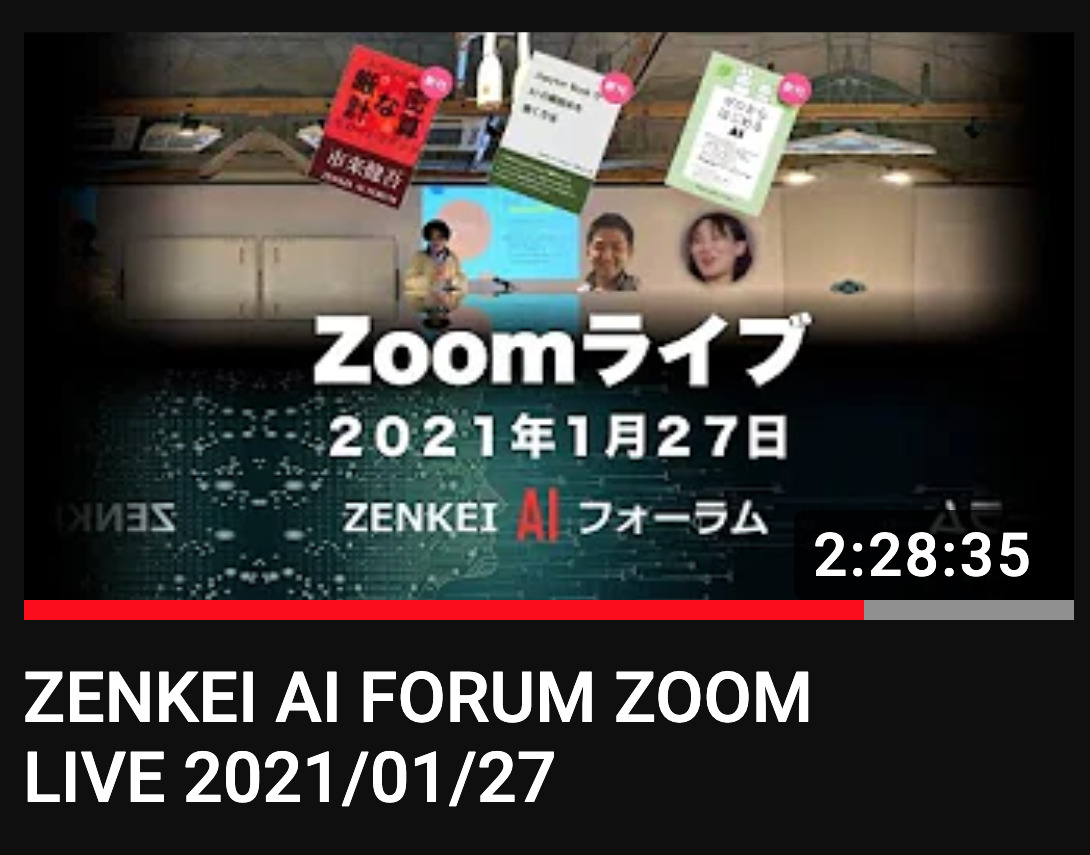
\includegraphics[width=0.45\textwidth]{images/202101/youtube.jpg}

内容は、以下の通りです。

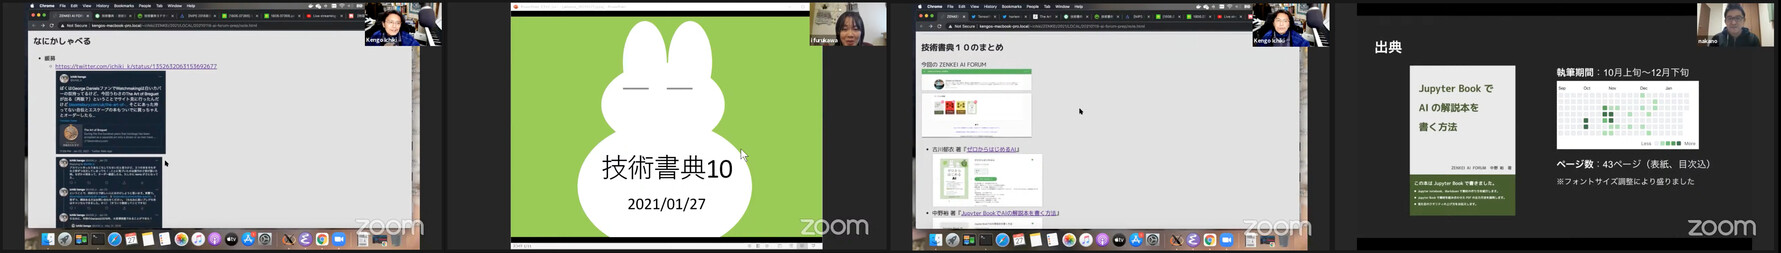
\includegraphics[width=0.45\textwidth]{images/202101/youtube-all.jpg}

\begin{itemize}
\item (前座)数理クイズじゃなくて、AI 関係の時事ニュース(市來)
\item 『技術書典10の報告、買った本の話、DALL・E』(古川)
\item 『技術書典10のまとめ』(市來)
\item 『Jupyter Book でAIの解説本を書く方法』(中野)
\end{itemize}

以下、
ZENKEI AI MAGAZINE (創刊号)2021年1月号のメイン・コンテンツとして、
発表者の3人にそれぞれ当日の発表内容をベースにして記事を書いていただきました。
お楽しみください。
\end{multicols}

\newpage

\chapter*{当日の発表内容(市來健吾)}
\addcontentsline{toc}{chapter}{当日の発表内容(市來健吾)}
\thispagestyle{fancy}
\AddToShipoutPictureBG*{%
  \AtPageLowerLeft{%
    \includegraphics[width=\paperwidth,height=\paperheight]%
      {images/p017-bg.jpg}
  }%
}%

2021年1月27日、今年最初の ZENKEI AI FORUM ZOOM LIVE では、
いつものようにイベント本番前の前座として、最近のぼくの身の回りの話題を紹介しました。
そのあと、メインの講演ではわれわれ「ZENKEI AI FORUM」サークル2回目となる
「技術書典10」への参加のまとめを発表しました。
以下、雑誌『ZENKEI AI MAGAZINE』の記事として、
内容をまとめたいと思います。

\vspace{0.45cm}

\begin{multicols}{2}
\subsection*{前座のはなし}
\addcontentsline{toc}{section}{前座のはなし}

\subsubsection*{緩募}
ぼくはよくオンラインで買い物をします。
主に本、最近はレコード・プレーヤーを買ったこともあり
少しずつレコード(LPというやつ、英語でいうところの vinyl ですね)を、
それも新譜を、買ってます。
そんな中、最近どういうわけか、手元に余分なものが届いたりしてます。
いろんな理由からメルカリとかヤフオクとか eBay とかで売りたくないし、
手元に置いててももったいないしと悩んでいる話を、
この日のイベントの前座、 icebreaker として話しました。

\subsubsection*{George Daniels の本}

みんさんは George Daniels という人物をご存知でしょうか?
ぼくは、いつだろう『Watchmaking』という大きくてきれいな本をみつけて
(もしかしたら 2000年前後の、まだ日本にいた頃だったかもしれない)、
それ以来、尊敬している人物の一人です。
いわゆる独立系の時計師と呼ばれるタイプの人で、
スクラッチからすべて懐中時計・腕時計を作り上げる人です。
イギリスの人で、数年前に既に亡くなっています。
ツイッターのタイムラインを見ていると、誰かが
「George Daniels の Breguet の本が復刻される」
という情報を上げていて、この手の本は最近特に、
出た時に入手しないと手に入らなくなるので、
すぐに調べて、イギリスの出版社で予約できることを知り、
早速注文しました。
その時、その出版社で出てる他の Daniels の本
(自伝と、エスケープメントの本)があったので、
併せて注文しました。

Breguet の本は(1万円以上する)まだ出版前だったけど、
他の2冊は既刊で、程なく出荷されたとの知らせがきました。
で、届いた箱を開けると中から2冊ずつ合計4冊の本が出てきました。
おかしいなと思って、オンラインの注文を改めて確認すると、
3種類の本をそれぞれ2冊ずつ注文してました。
ここは出版社独自のオンライン・サイトで、注文に際しアカウントを作ったりして、
ページを行ったり来たりしたせいで(?)2冊注文になってしまったようです。
これがドル建てだったら確認時にピンと来たんでしょうが、
ポンドは感覚的によく分かってなかったのもいけませんでした。

国際郵便で届いたものなので、返品するから返金してというのも大変だと思いましたが、
Breguet の本は高いし未発送なので「一冊の注文はキャンセルして欲しい」
というメールを書いたところ、快く対応してもらい、ほっとしました。
本来、ぼくの注文ミスだったし。

しかし、この手元に余分に余った2冊の本、ぼくの手元で飾りになっているよりは、
どこかの同好の士に喜んでもらえればいいな、という話です。

\subsubsection*{AI は流体力学を解けるのか?}
一時期、AI がみんなの仕事を奪ってしまうと言ってみんな騒いでいました。
そこで言われていた「仕事」というのは単純作業などで、
人間の創造性に関する仕事は大丈夫だ、というノリでした。
(そういえば、すっかりそういう話を聞かなくなりました。
\ruby{流行}{はや}りというのは廃れるのも早いですね。
そういう意味でも、流行からはやはり一線を引いておきたいなとぼくは思います。)

\AddToShipoutPictureBG*{%
  \AtPageLowerLeft{%
    \includegraphics[width=\paperwidth,height=\paperheight]%
      {images/bg-light-blue.png}
  }%
}%

一方で、これはぼくの最初の同人誌『音楽と数理』の最後に載せた、
元々は Qiita に書いた記事『グーグルMagentaの採譜プログラムと自分のプログラムを比べたら互角の勝負だったという話』
(\url{https://qiita.com/kichiki/items/0325aa2e8b70416f6597})
でもコメントした話ですが、
Computer Vision という分野は、その多くが今や Deep Learning によって
取って代わられました。
今時オブジェクト認識するために SIFT 特徴量とか Hough 変換を計算したりしませんよね。
この Qiita の記事では、ぼく自身、画像処理においては
Deep Learning に転向した人間であるにもかかわらず、
記事の主題である音楽の解析においては、 Google Magenta チームが開発した
Deep Learning によるアプローチを\ruby{由}{よし}としない、
ちょっと矛盾した気分を味わったと書きました。

そんな中、最近目にしたツイート
(\url{https://twitter.com/yellowshippo/status/1352092313497997315})
で「流体力学を Deep Learning で解こう」という話を見かけました。
言及されていた論文は
``Learning Incompressible Fluid Dynamics from Scratch
-- Towards Fast, Differentiable Fluid Models that Generalize''
(\url{https://arxiv.org/abs/2006.08762})
です。
実はぼくは、本職は(というと語弊がありますが、
今のプログラマー稼業に就く前は)
物理学、その中でも流体力学の理論および数値解析に関する研究者でした。
言ってみれば、この話題において AI に職を奪われる側ということになります。

この論文とは直接関係ないですが、
このご時世、最近(昔のぼくのような)物理学者がツールとして Deep Learning を
使い始めているようです。
DeepMind が宣伝してるタンパク質の折り畳みの話など、その一例です。
しかし、心情的にも、また多少は物理にも AI 側にも経験を持った人間としても、
物理の研究、特に理論や数値解析の領域に AI を使う姿勢というのは、
なにかまだ素直に受け入れられないものがあります。
かつてシビアな数値解析屋の立場に立っていたとき、
リアルの実験家がうらやましいと思うことが時々ありました。
実験家は気楽でいいよな、全てを知っている「自然」に素直に問いかけて
答えを聞けばよいのだから、と。
(もちろん実験の難しさは全て棚に上げて言っている八つ当たりみたいなものです。)
Deep Learning や Machine Learning で、
いわゆる教師あり学習の枠組みを使って、
数値シミュレーションを行ったり、
近似モデル(のパラメータの最適化)をやるのは、
理論家の仕事というよりはむしろ実験家の仕事だと感じます。
一方で AI 手法といえども突き詰めれば一種の数値ソルバーであり、
最適化問題を解くたくさんの手法のなかの1つに過ぎないのだから、
そんなに過敏になる必要はないという気分もあります。
しかし、ではその立場で AI を使おうとしているのだとすると、
それってなんだか新しい測定装置が手に入ったので使ってみただけのように見えてしまいます。

実のところ Deep Learning というのは
ちょっと気の利いた柔軟性に富む数値ソルバーに過ぎないのでしょうか?


\subsection*{技術書典10のまとめ}
\addcontentsline{toc}{section}{技術書典10のまとめ}
今回の「技術書典10」は、われわれ「ZENKEI AI FORUM」としては2回目の参加で、
前回の2冊から、4冊へと出典書籍が増えました。
以下が最終的な今回の「技術書典10」への ZENKEI AI FORUM サークルの
出典ラインナップです。

\begin{itemize}
\item 古川郁衣 著『ゼロからはじめるAI』\\
  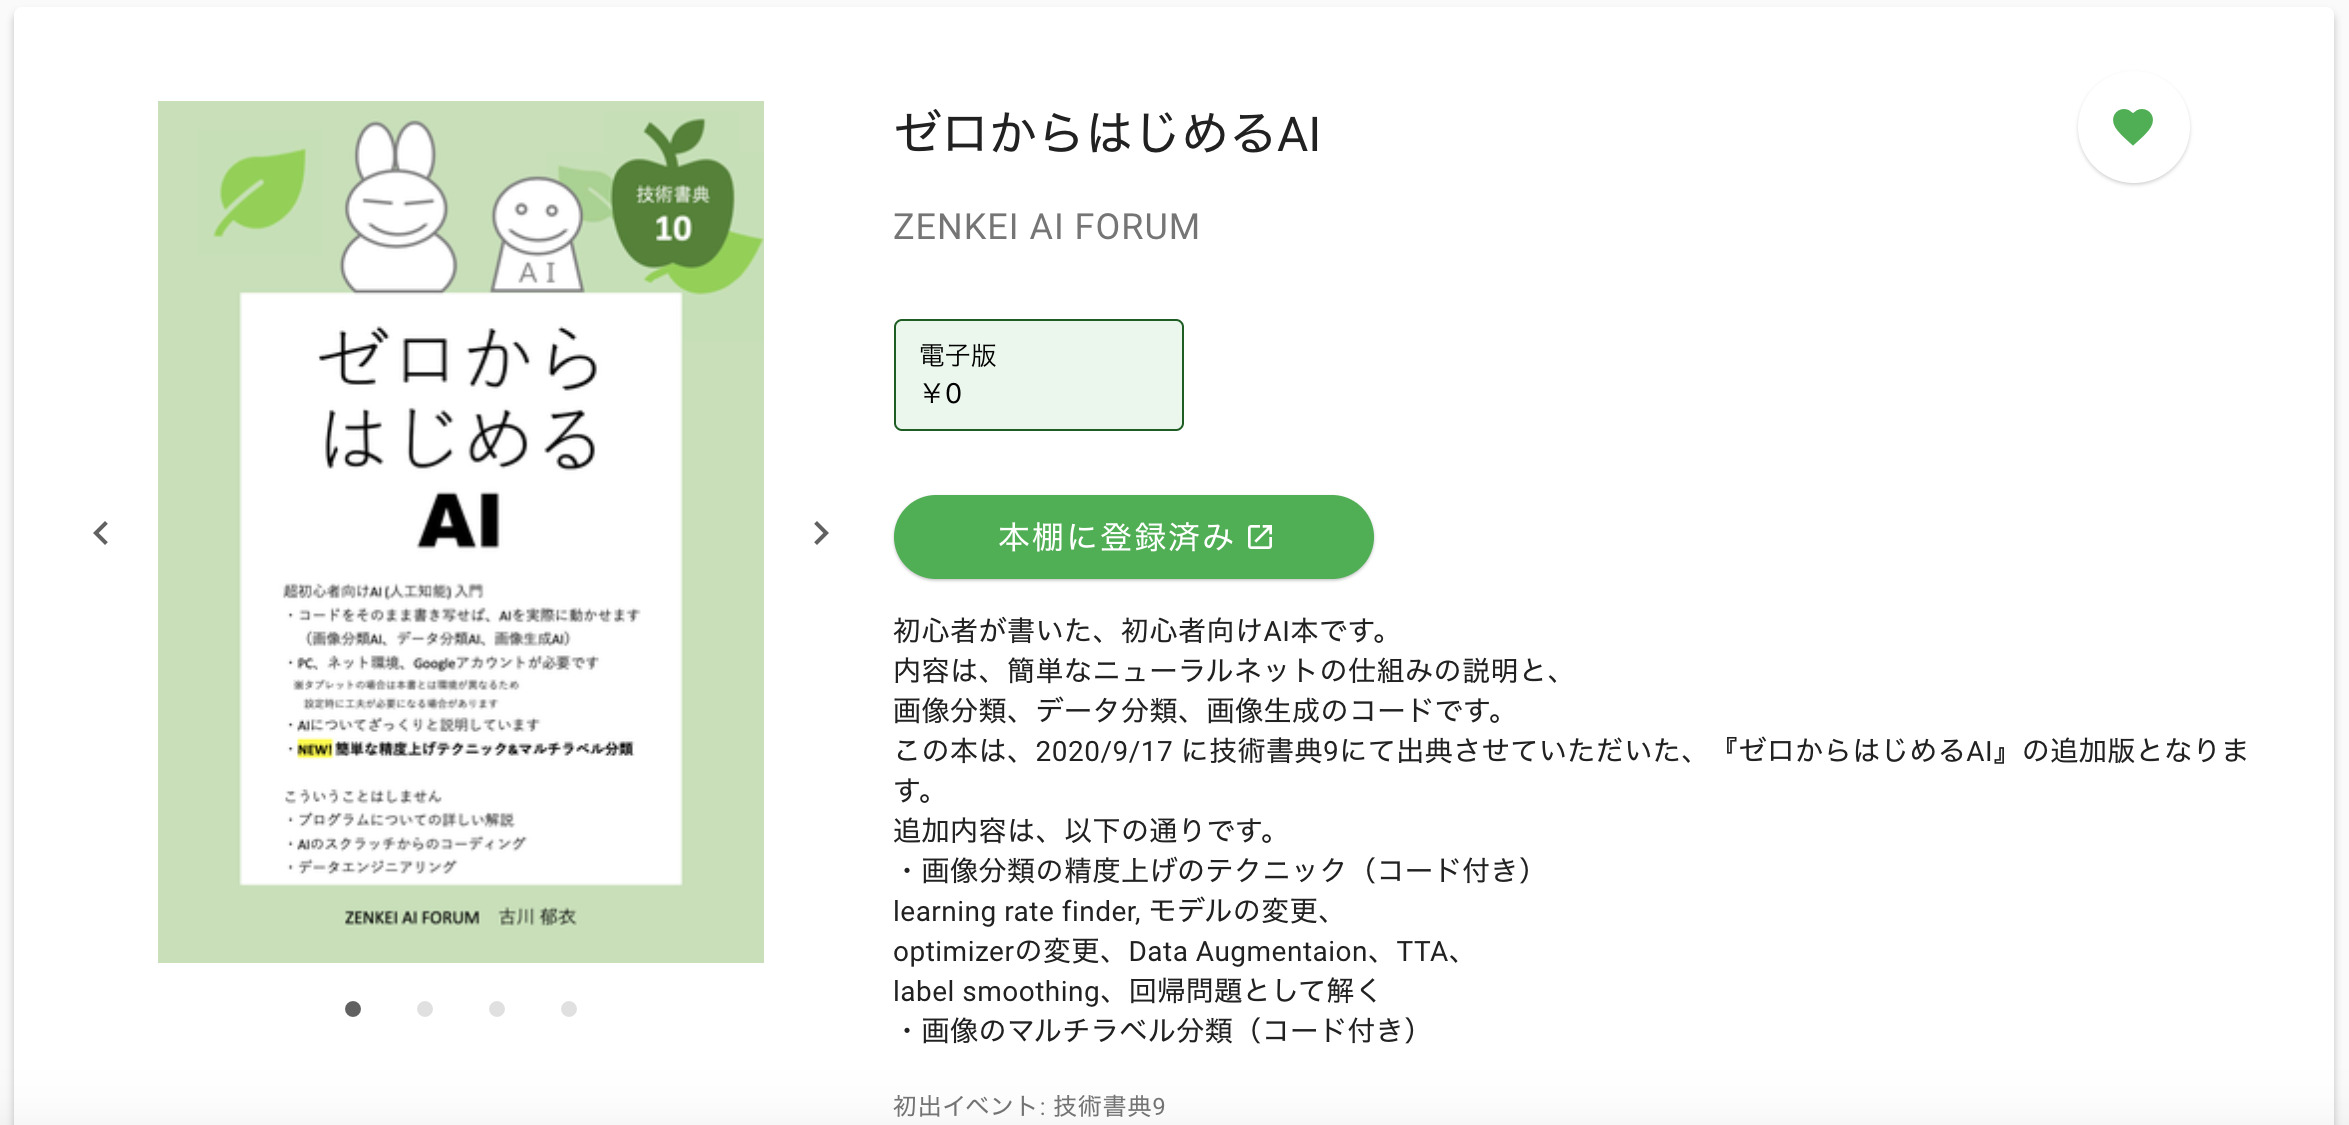
\includegraphics[width=0.45\textwidth]{images/202101/techbookfest-10-furukawa.jpg}
\item 中野裕 著『Jupyter BookでAIの解説本を書く方法』\\
  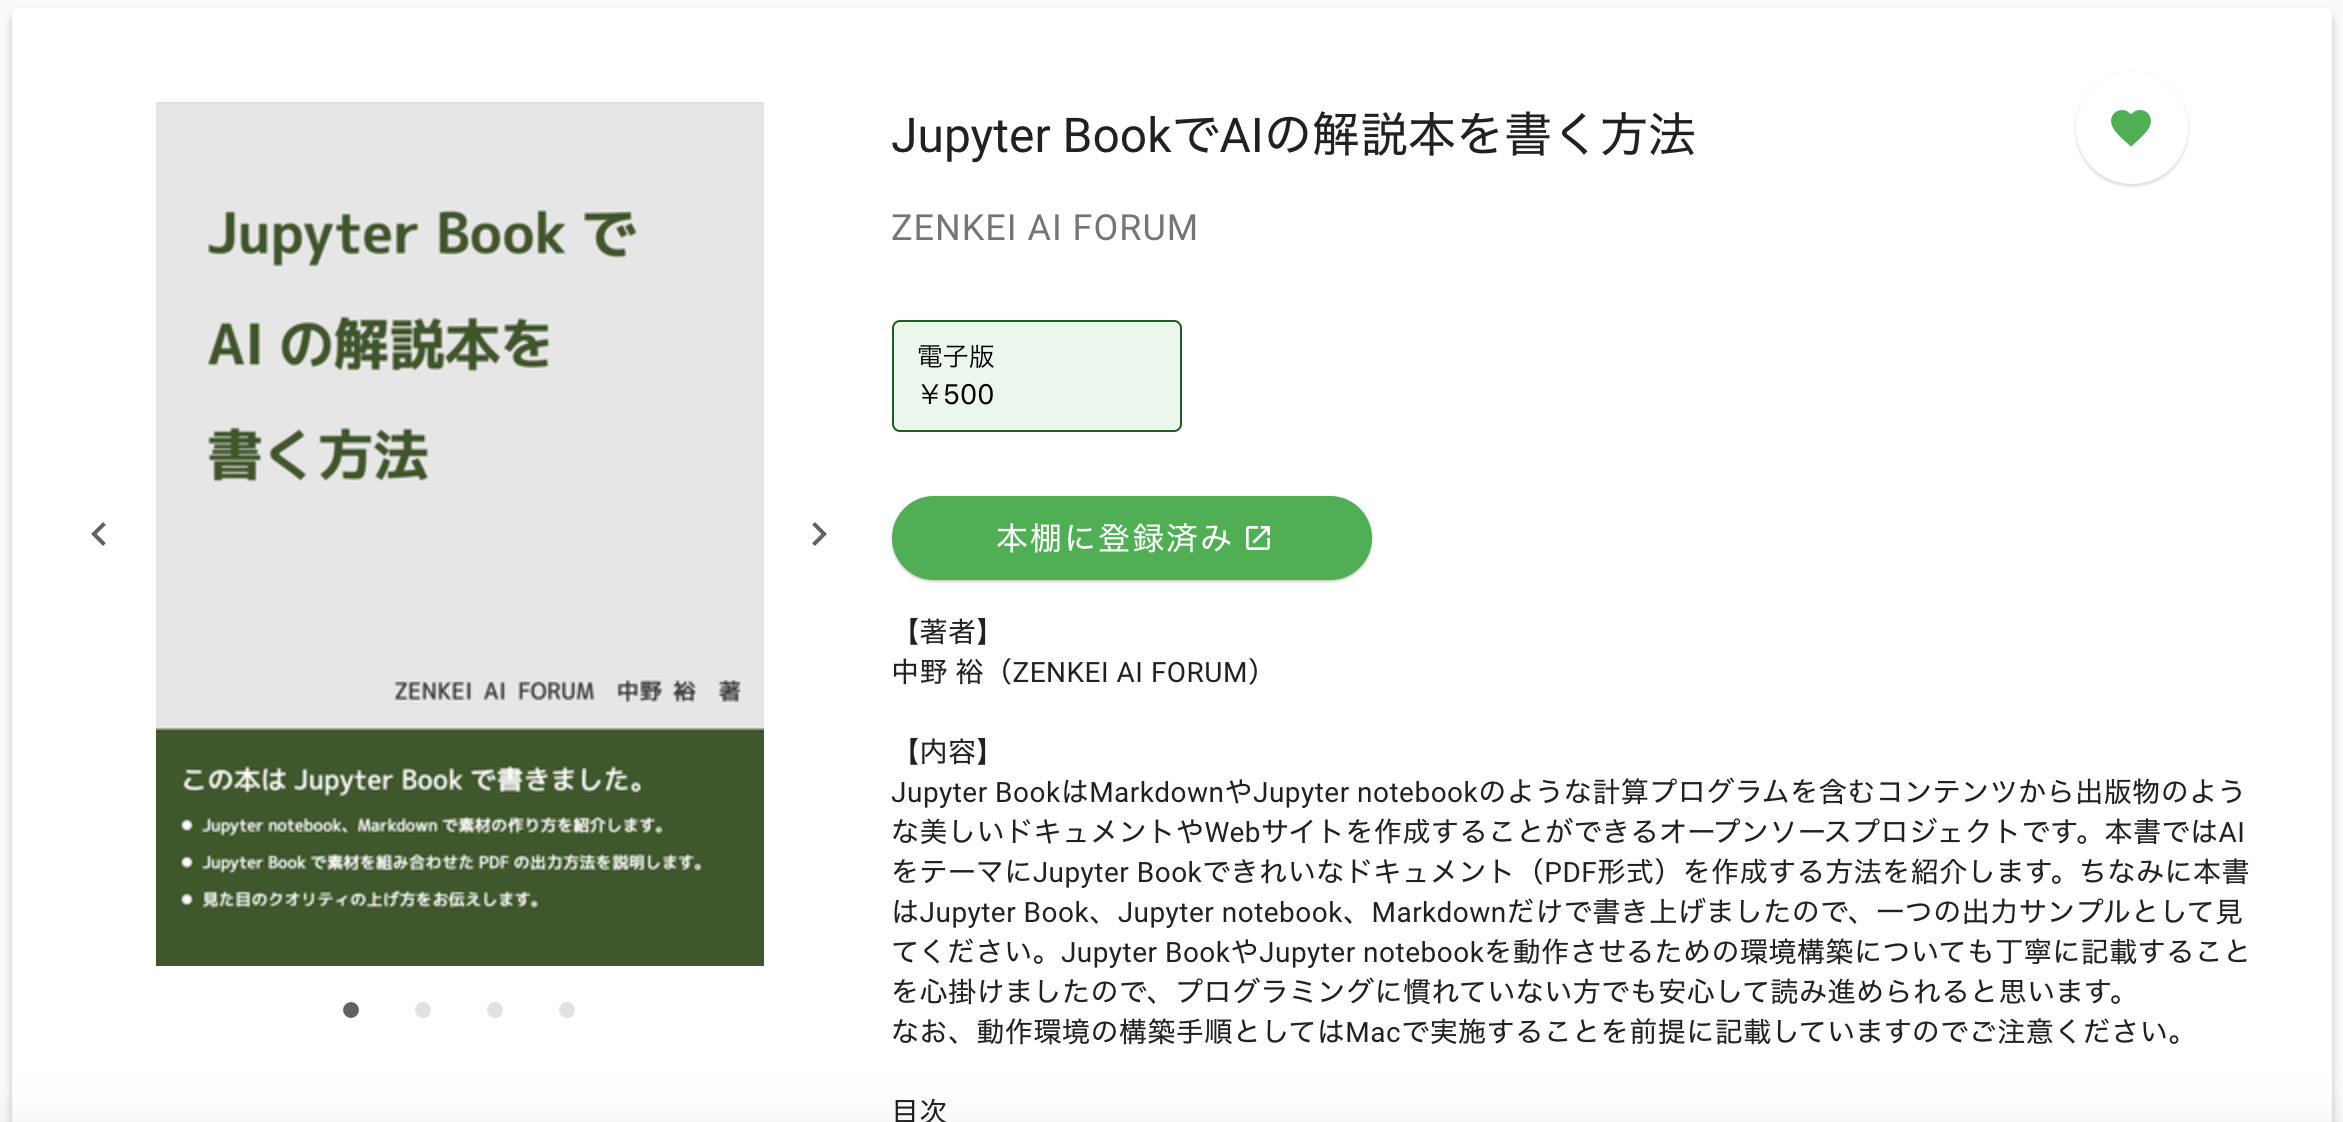
\includegraphics[width=0.45\textwidth]{images/202101/techbookfest-10-nakano.jpg}
\item 市來健吾 著『音楽と数理 才能にたよらない耳コピ』\\
  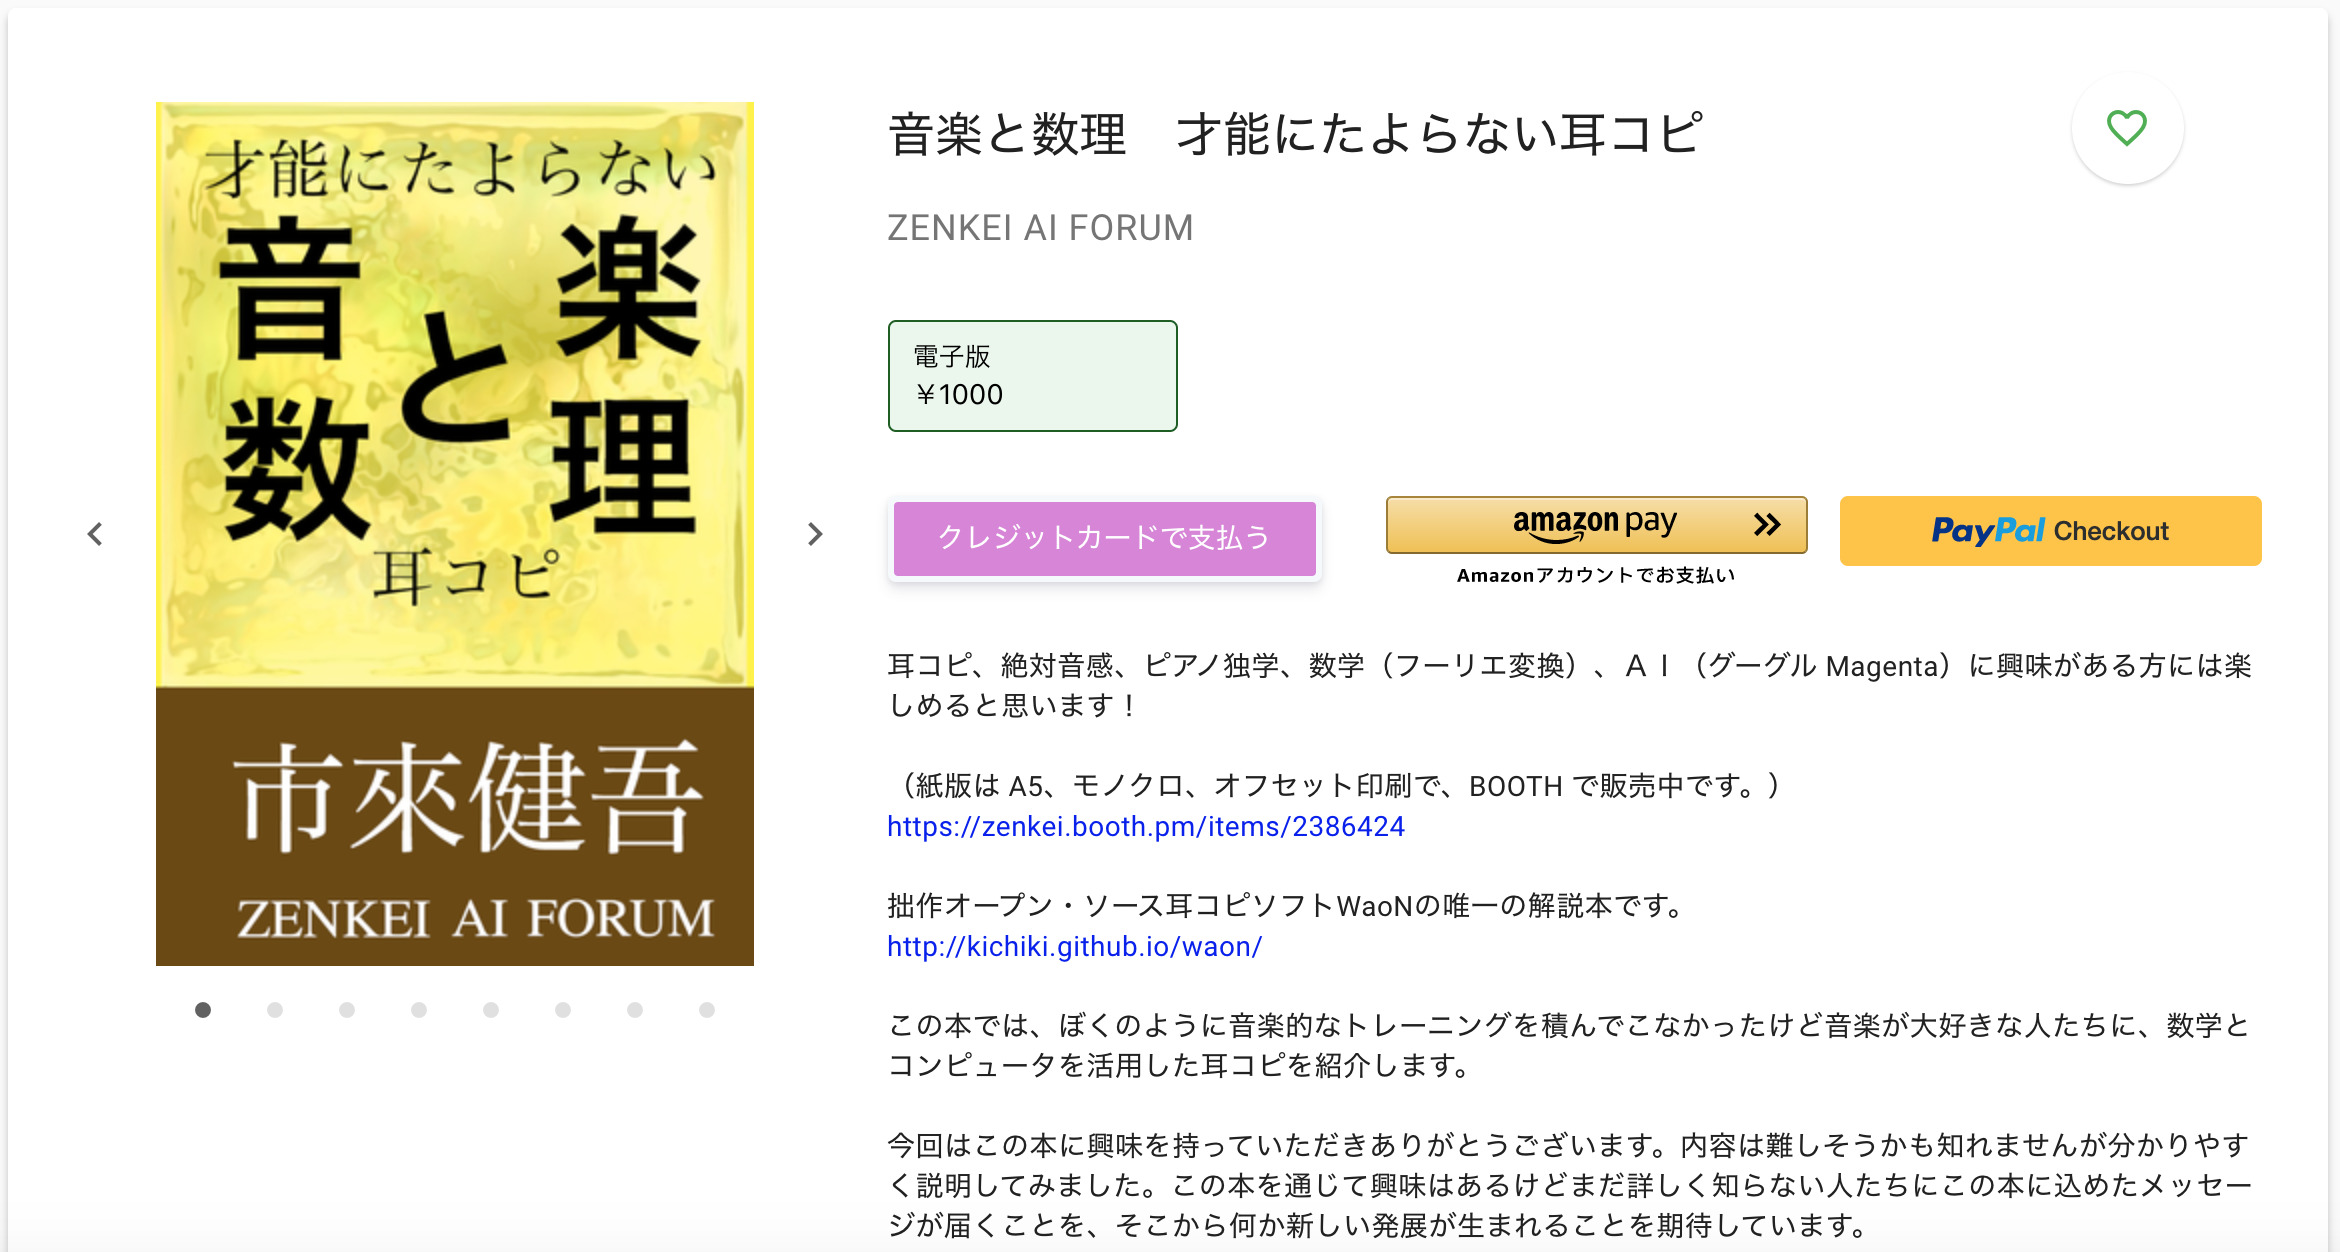
\includegraphics[width=0.45\textwidth]{images/202101/techbookfest-10-ichiki-1.jpg}
\item 市來健吾 著『厳密な計算 ふたつの球のなめらかなダンス』\\
  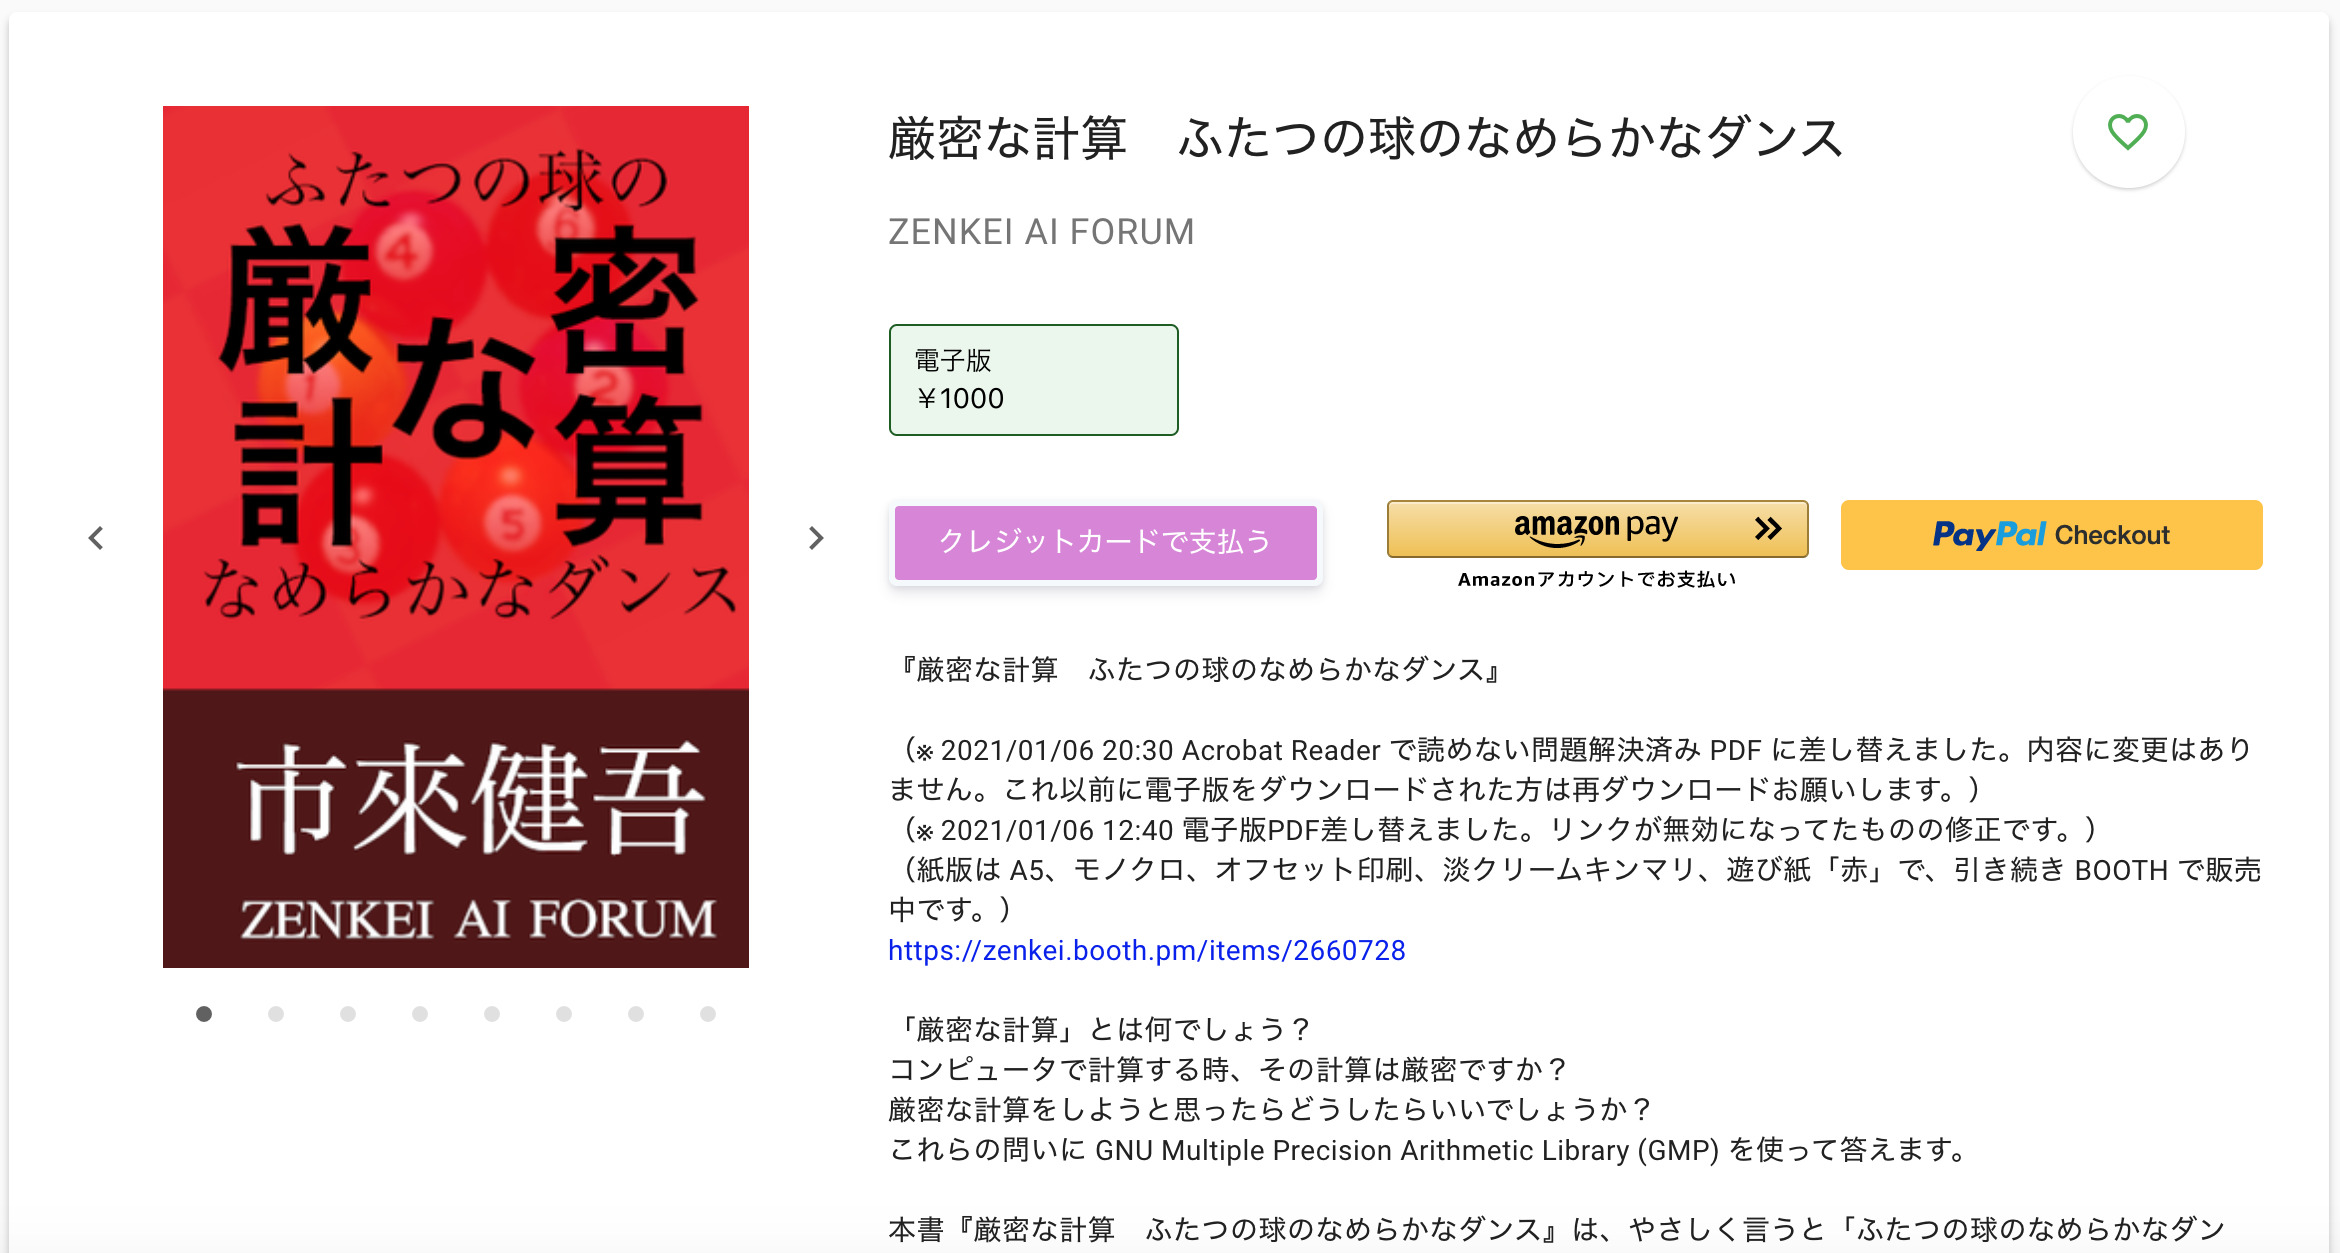
\includegraphics[width=0.45\textwidth]{images/202101/techbookfest-10-ichiki-2.jpg}
\end{itemize}

ぼくの執筆に関しては、
今回は、既刊『音楽と数理』を引き続き出典し、
さらに新刊『厳密な計算』を書き下ろしで1冊、
計2冊の出典としました。

\AddToShipoutPictureBG*{%
  \AtPageLowerLeft{%
    \includegraphics[width=\paperwidth,height=\paperheight]%
    {images/bg-light-blue.png}
  }%
}%


前回「技術書典9」のふりかえりを、
Qiita (\url{https://qiita.com/kichiki/items/6d14c7bfea7ef95f4e1a})
に投稿しましたが、

\begin{quotation}
  およそ20日間で1冊の本『音楽と数理』を書き上げて、出典したドタバタ
\end{quotation}

と書いた通り、かなりの修羅場でした。
9月にイベント終了に際し「次回は12月」とのアナウンスがあった時、
3ヶ月あれば、今度はじっくり執筆できるな、と考えていました。
しかし蓋を開けてみると、どうも何も学んでいなかったようです。
以下、2020年12月6日のツイート(\url{https://twitter.com/ichiki_k/status/1335475252017549313})からの引用です。

\begin{quotation}
  予告してましたが拙著、数理三部作構想の2冊目『厳密な計算』ようやく手を動かし始めました!と思ったら \#技術書典 10 までもう3週間を切りましたね(何も学んでない→ \url{https://qiita.com/kichiki/items/6d14c7bfea7ef95f4e1a} )
\end{quotation}

(原文ママ)

その後、紆余曲折の末、イベント開始を過ぎた2020年の大晦日、
なんとか出典できました。

\vspace{1em}
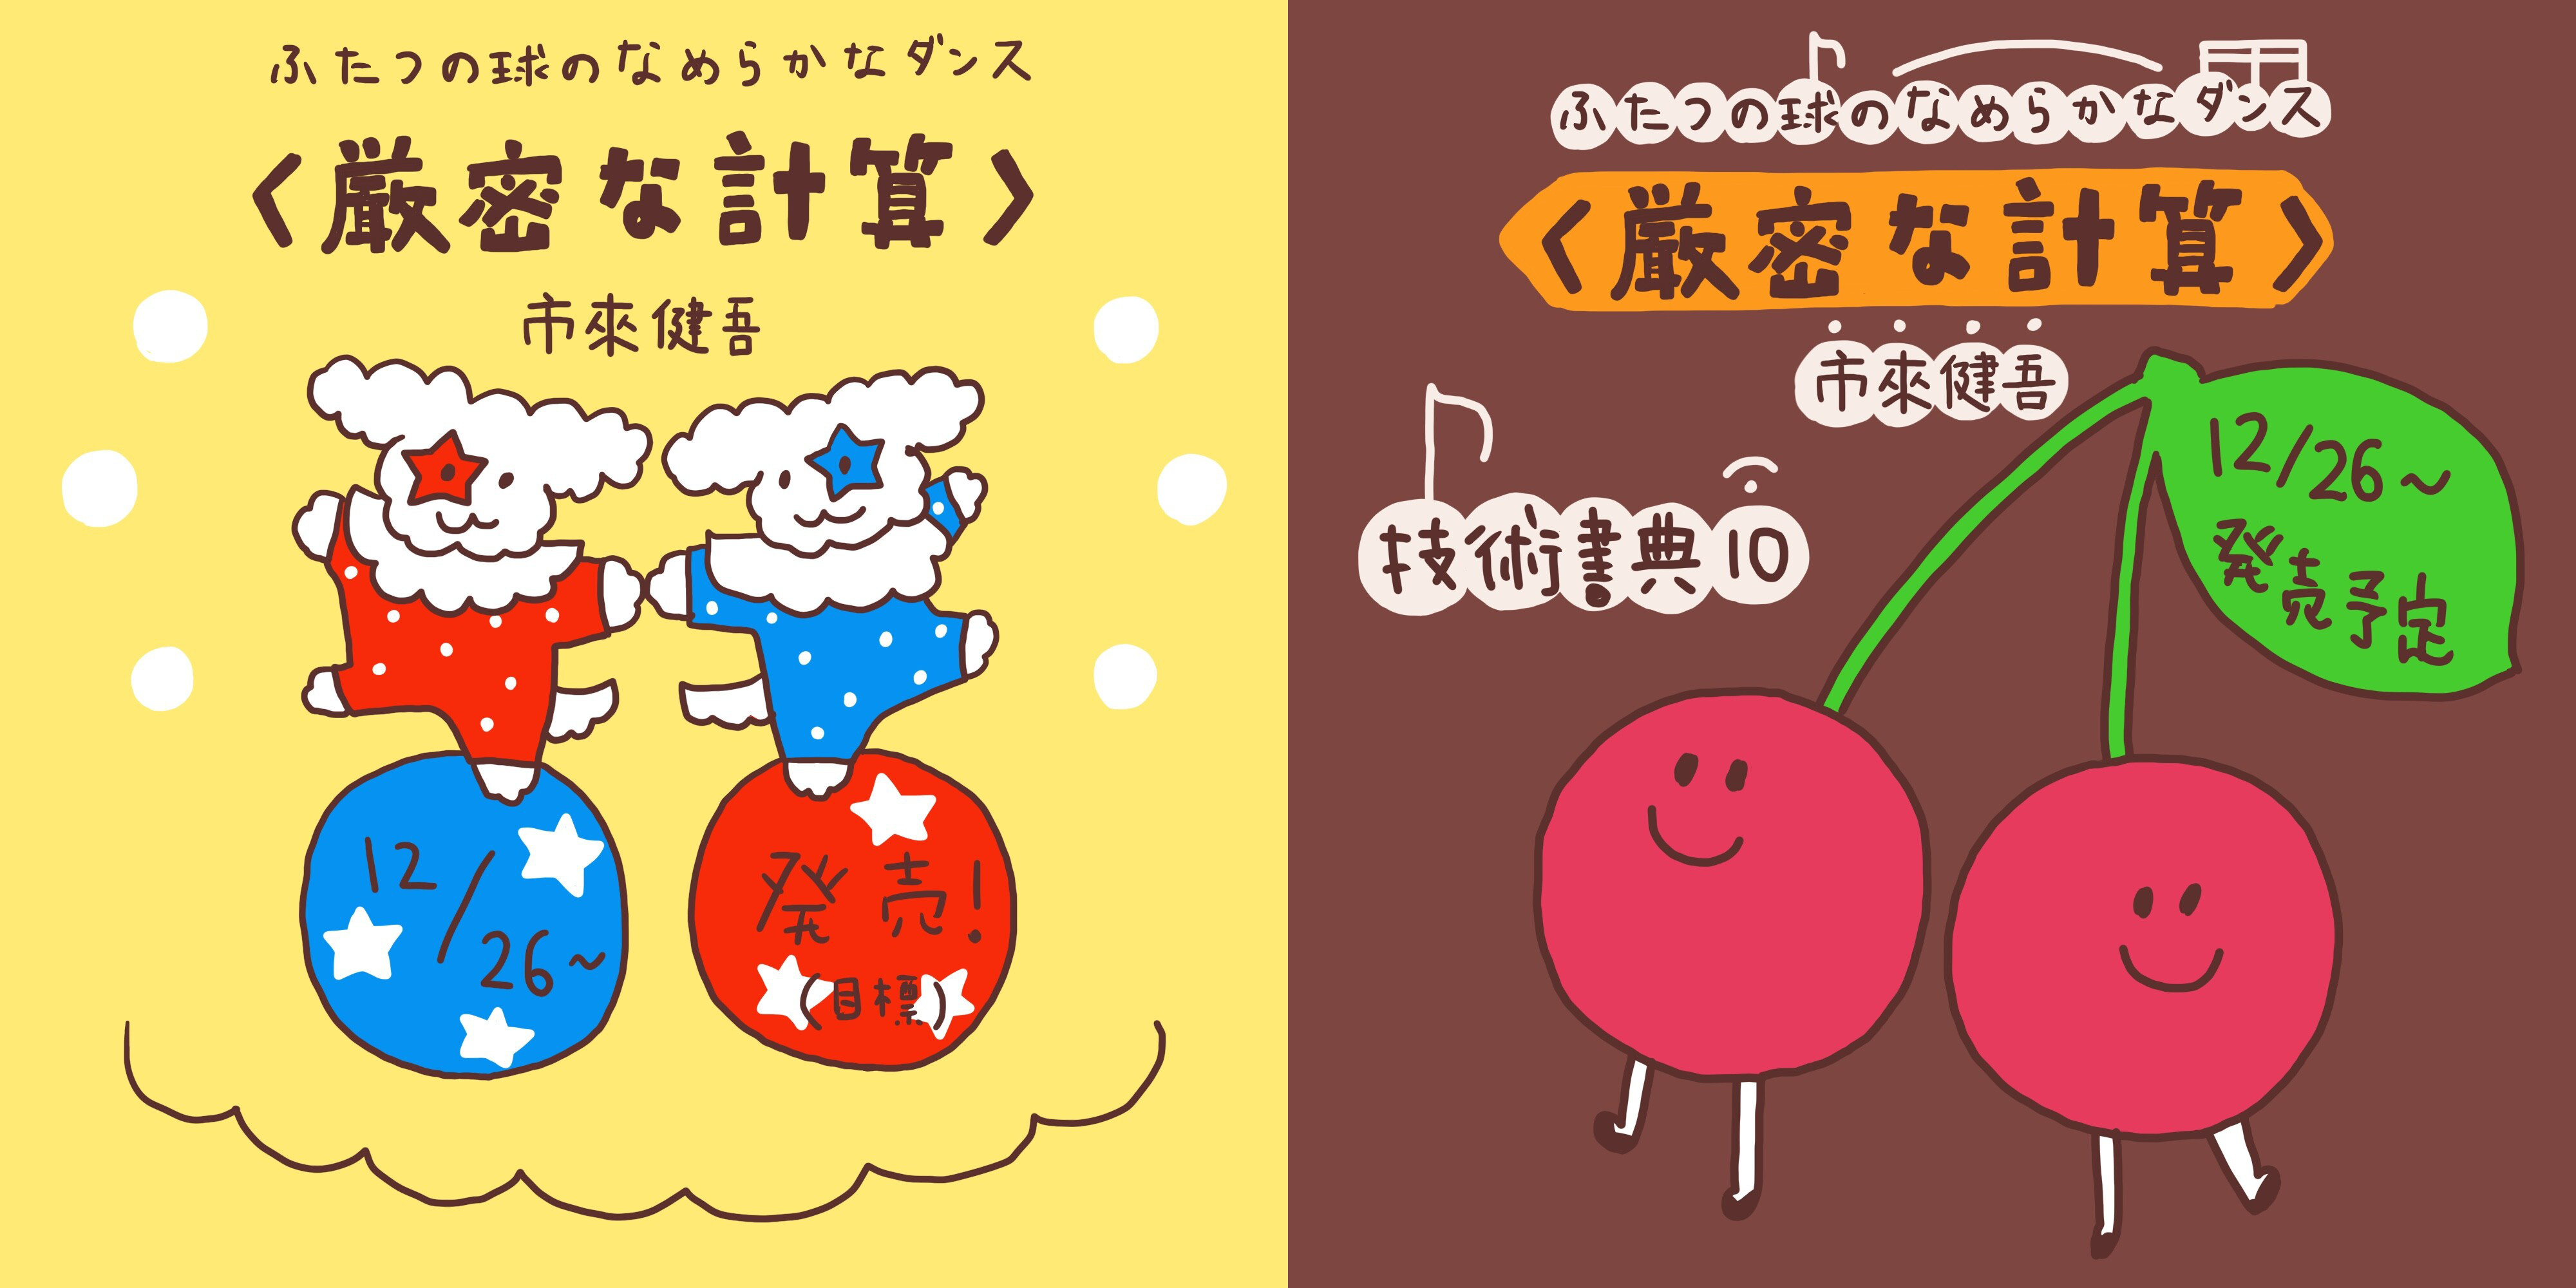
\includegraphics[width=0.45\textwidth]{images/202101/exact-computation-furukawa.jpg}
\begin{center}
  {\small 古川さんに事前に描いてもらっていたイラスト}
\end{center}
\vspace{1em}

今回も、また、紙の本を印刷しました。
前回同様、日光企画さんに頼みました。
2回目になると、いくつか改善したい点や試してみたいことが出てきます。
それは紙の選択と、遊び紙という表紙裏に入れることができる色紙です。
印刷された本が自宅に届いたときのツイート
(\url{https://twitter.com/ichiki_k/status/1350112024462651393})
を引用します。

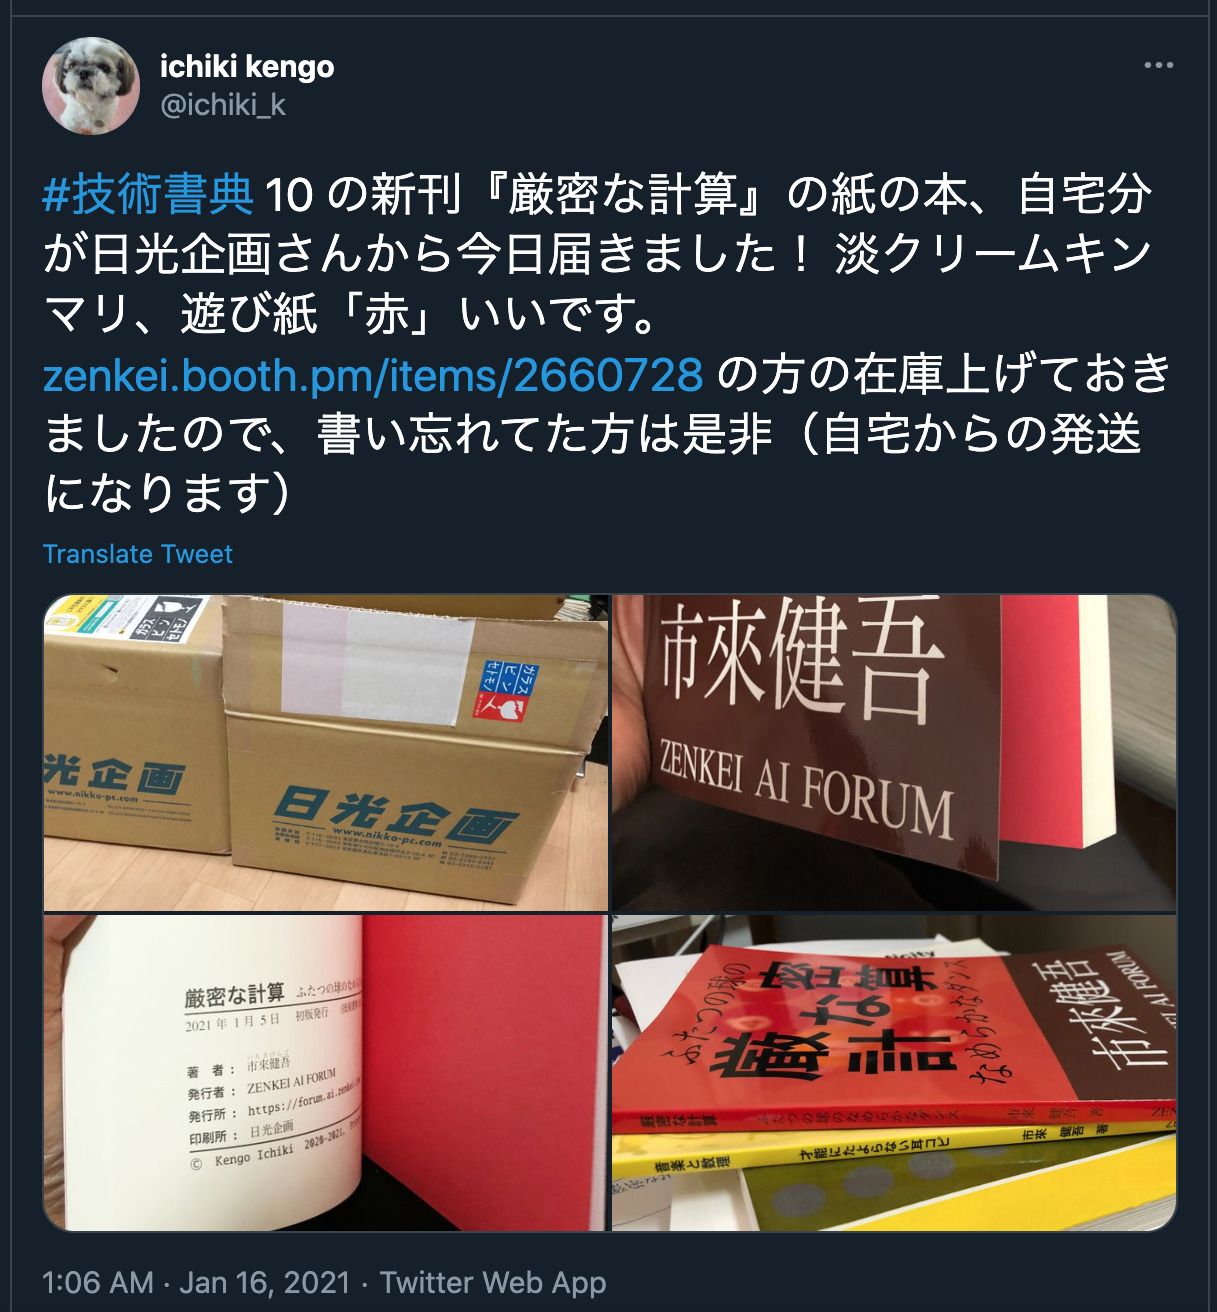
\includegraphics[width=0.45\textwidth]{images/202101/tweet-exact-computation-book.jpg}

ご覧の通り今回は紙を「淡クリームキンマリ」、遊び紙は「赤」にしてみました。
とても満足しています。

\AddToShipoutPictureBG*{%
  \AtPageLowerLeft{%
    \includegraphics[width=\paperwidth,height=\paperheight]%
      {images/p020-bg.jpg}
  }%
}%

\subsubsection*{今後}
今回の「技術書典10」でのサークル「ZENKEI AI FORUM (ZAF)」の
書籍ラインナップを改めて見なおして、
AI を広めたいというフォーラムの趣旨を考えても、
実際に ZENKEI AI FORUM のイベントから生まれ書籍化された『ゼロからはじめるAI』と、
同じくフォーラムで声かけして中野さんが書いてくれた
『Jupyter BookでAIの解説本を書く方法』と、
この2冊こそが ZAF の本としてふさわしいと思いました。
対してぼくの書いた2冊は(最初から、自分の持ちネタを形にしたと断ってはいましたが)
AI との関連も弱く、ちょっと場違いかなと感じました。
なので将来的にはこの2冊はラインナップから落とすことにしようと考えています。

ただそれだと ZAF の同人誌活動の後退だと思うし、それは残念なので、
穴埋めではないですが何か代わりに出来ることはないだろうかと考えました。
そして ZENKEI AI FORUM の雑誌があってもいいんじゃないか、と思いました。
というより同人(サークル、秘密結社)といえば
何は無くとも「雑誌」でしょう、と。

ということで『ZAM』創刊します(というか、しました)。
\end{multicols}


\newpage

\chapter*{ }
\addcontentsline{toc}{chapter}{技術書典10報告 (furukawa)}
\thispagestyle{fancy}
\AddToShipoutPictureBG*{%
  \AtPageLowerLeft{%
    \includegraphics[width=\paperwidth,height=\paperheight]%
      {images/p021-bg.jpg}
  }%
}%

\begin{tikzpicture}[remember picture, overlay]
  \node[xshift=0cm,yshift=-4.2cm] at (current page.north){
    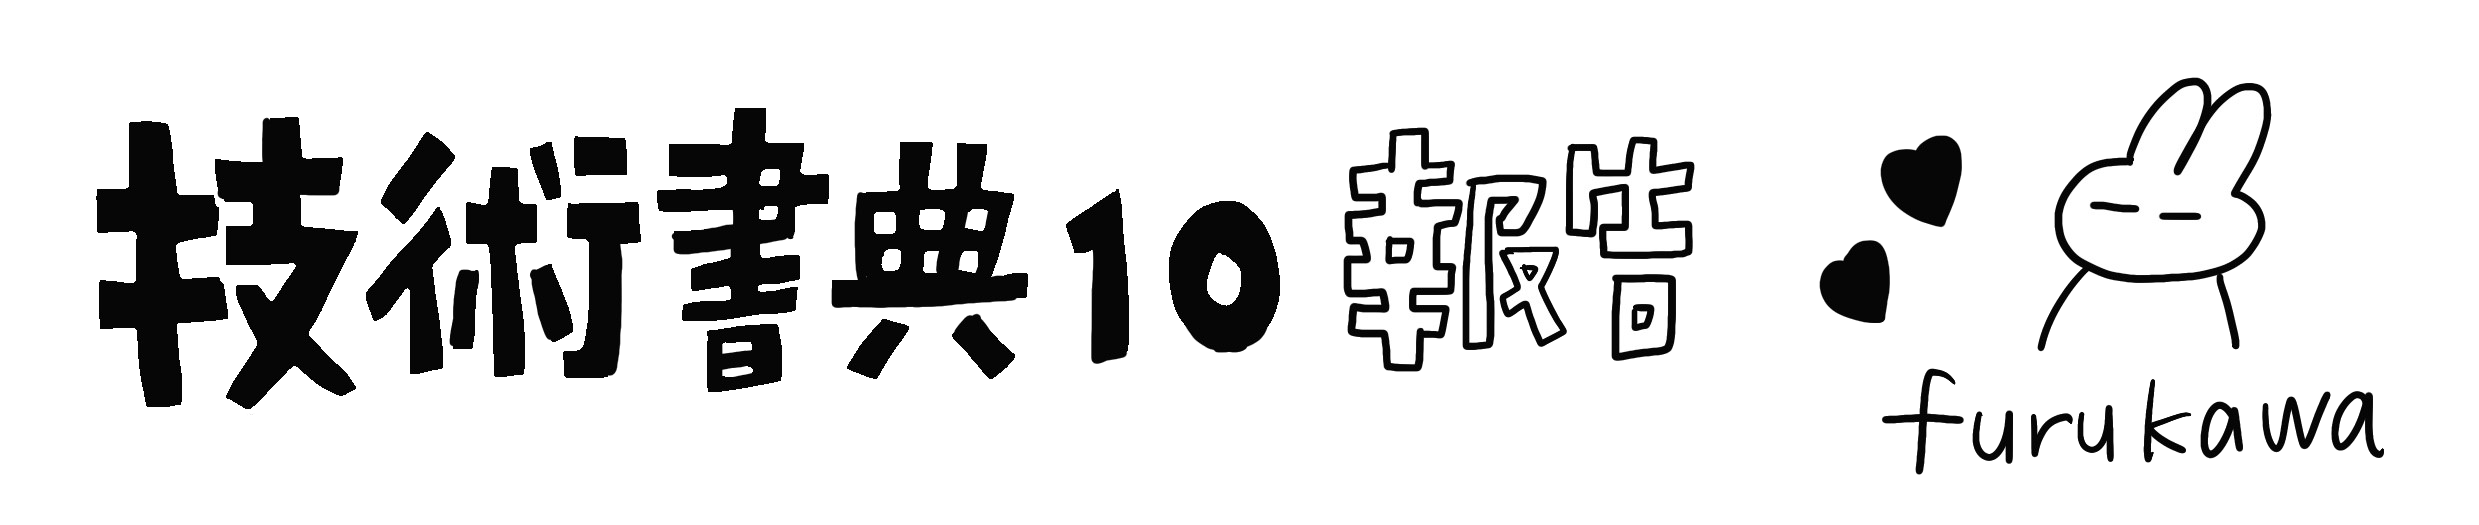
\includegraphics[width=1.2\textwidth]{images/202101/newsletter202102.png}
  };  
\end{tikzpicture}

\begin{multicols}{2}

\subsection*{概要}
\addcontentsline{toc}{section}{概要}
\begin{itemize}
\item 技術書典10(2020/12/26~2021/1/6)への参加報告
\item 技術書典10で購入した本の紹介
\item* DALL・E
\end{itemize}

\subsection*{技術書典10(2020/12/26 -- 2021/1/6)への参加報告}
\addcontentsline{toc}{section}{技術書典10(2020/12/26 -- 2021/1/6)への参加報告}
今回は、前回出典した『ゼロからはじめるAI』(\url{https://techbookfest.org/product/6566174659706880})への追記をした本と、個人で趣味の本を出しました。どちらも無料で出しまして、『ゼロから~』のほうは400冊、趣味の本は80冊ほどダウンロードが出ました。Qiitaで無料本まとめの記事がたくさん見られていたようですので、そこから来てくださったかたがかなりいたのかもしれないです。もし私個人が電子書籍を作ってSNSに告知しただけであれば到底出ない数です。今回は年末年始の開催で出典者が前回より少なかったようですが、それでもイベントをチェックしている人の多さを感じました。
 
\end{multicols}


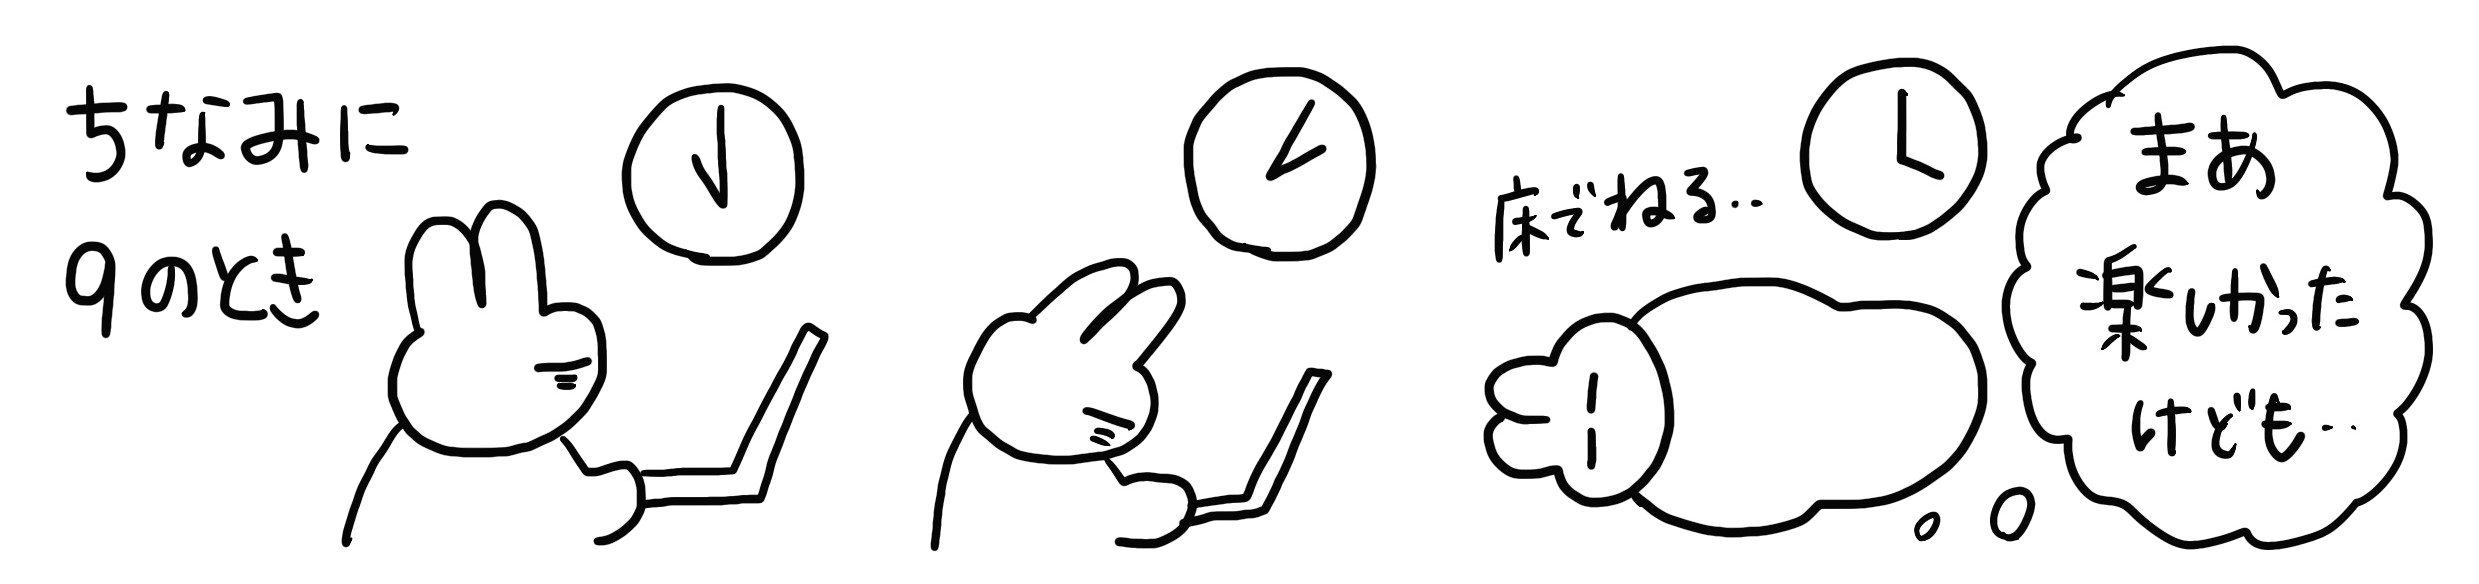
\includegraphics[width=\textwidth]{images/202101/newsletter202102_1.png}
\begin{center}
  ※技術書典9のときは毎晩夜中に作業していたので、作家気分を味わいました(?)。
\end{center}


\begin{multicols}{2}
『ゼロから~』に関しては前回20日程度で1冊を書き起こすというかなり無茶なスケジュールで大変でしたので、今回は2か月ほど前から内容を用意しており、比較的楽でした。前回ニューラルネットの説明といくつかのモデルのコード紹介をしたので、モデルの精度上げのテクニックについて追記しました。

\end{multicols}


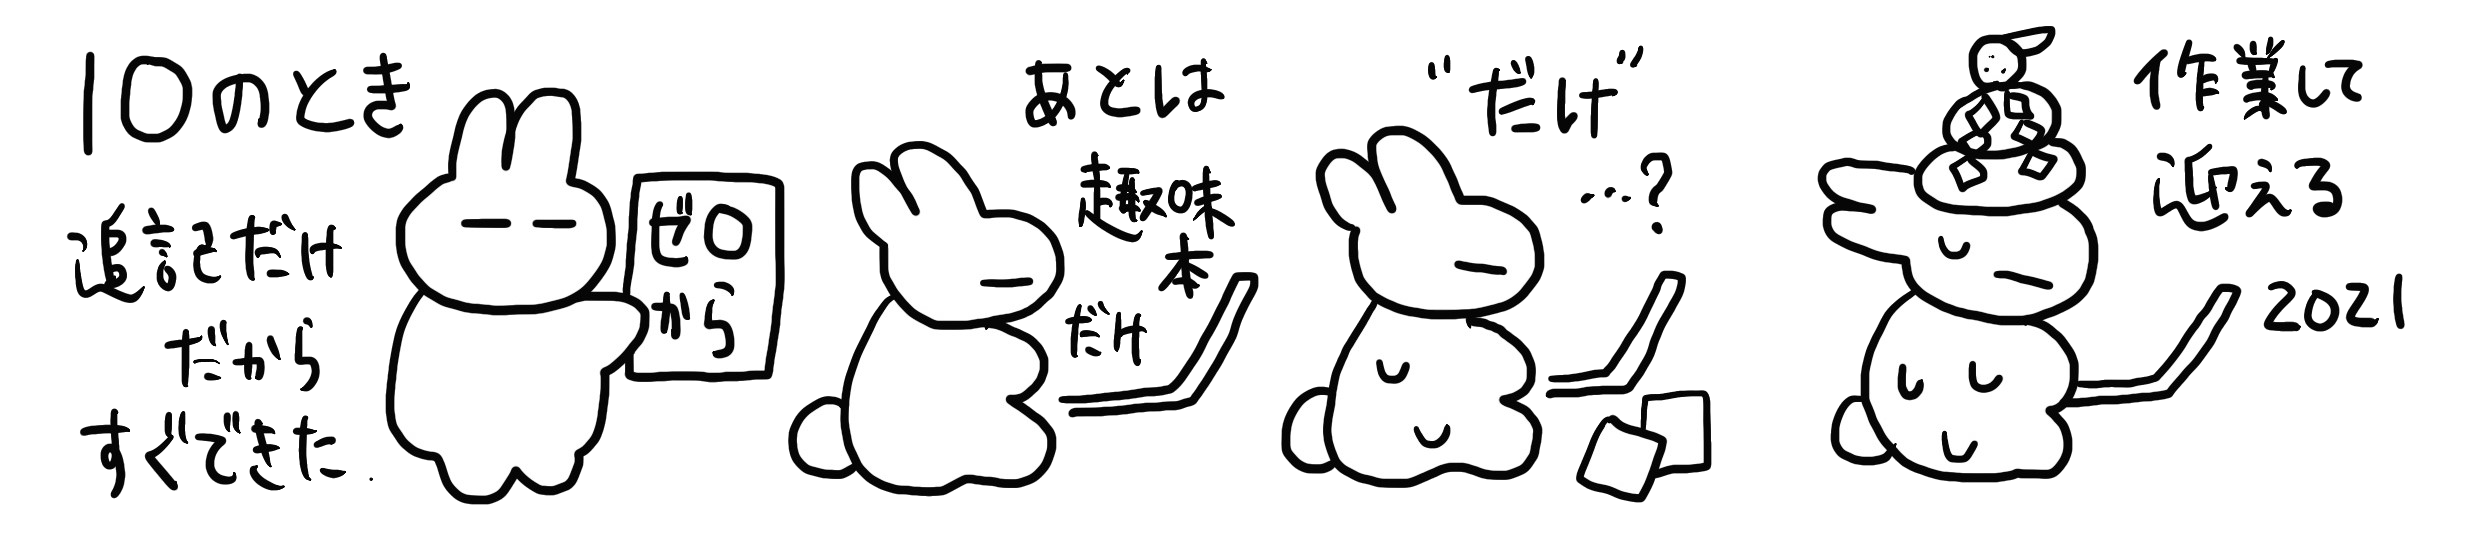
\includegraphics[width=\textwidth]{images/202101/newsletter20210218_2.png}


\begin{multicols}{2}
趣味の本のほうは、内容が趣味すぎて、技術書典に来るようなエンジニアの人には読まれないのではと思っていましたが、物珍しさもあったのか、意外と読んでいただけたようです。これを書く際、掲載する作品も同時に作らなくてはならなかったので結局イベント開始日に間に合わず、年もまたぎ、1/4にようやく出典できました。

デザインもレイアウトも自由なので楽しかったです。次回への反省点を記載しておきます。

\subsubsection*{電子書籍作成反省点}

\begin{itemize}
\item iPhoneで撮った写真をそのままたくさん貼りつけたのでPDFが重くなってしまいました。事前にまとめてサイズを小さくしておくべきでした。
\item マンガやイラストなどの遊び要素をもっと入れたかったです。
\end{itemize}


自分でサークルを作って出典したので、そのことについて記録しておきます。

\subsubsection*{超かんたん!サークル初出典手順}

\paragraph{\gtfamily\bfseries ■サークル結成}

個人でも出典できるので、出ると決めた時点で結成完了です。

\paragraph{\gtfamily\bfseries ■サークル申請}

申請受付期間中に技術書典のサイトから申し込みをします。このとき、出典する本の概要と、サークルの活動内容が分かるサイトかSNSのリンクが必要です。私は趣味のサイトもSNSアカウントも何も持っていなかったので、Instagramのアカウントを作り、そこに作品を載せました。やっつけすぎて通らないのではないかと思いましたが、数日後に問題なく参加許可が出ました。ただ、次回からはlinktreeのリンクで申請しようと思います。linktreeはSNSなどのリンク先を1ページに表示するためのサービスで無料で利用できます。

\paragraph{\gtfamily\bfseries ■電子書籍作成}

反省点は先のページに書きました。

PDF/EPUB/ZIPのいずれかで提出することになっているので前作同様、PowerPointで作りました。パワポ?!と思われるかもしれませんが、操作が簡単でレイアウトが自在だしある程度数式もかけるので、今の私にはこれで十分なんです。

PCで見ることを考慮し、画面上で見開きでみてほしいこの本は横長にしました。技術書典では縦長サイズが前提みたいで、書典に並んだときに横幅に合わせて表示サイズが少し小さくなりましたが、そのほかは問題ありませんでした。

\paragraph{\gtfamily\bfseries ■書籍申請}

書籍ができたら、技術書典のサイトから申請します。ドラッグ&ドロップで完了です。UIが分かりやすいので、特に迷うことはありませんでした。

翌日くらいにはOKが出て、作った本が書典に並んでいました。技術書典の運営さんががんばってチェックしてくださっているようです。本当にごくろうさまです。
技術書典の自分の本のページにはサンプル画像を上げられるようになっています。普通は目次や本の一部を載せるものですが、私は追加で、このページまで来てくれた人へのサンキューレターを載せていました。これを次回は毎日変えたいです。そのほうが絶対楽しいと思います。

\paragraph{\gtfamily\bfseries ■本紹介イベント参加}

趣味本に関してはできあがったのが遅すぎて参加できなかったのですが、運営の方が本の紹介イベントを行っているので、次回は参加したいです。

書いたものをPDF出力できる仕組みさえあれば、それで電子書籍を作って参加することができるので、興味を持たれたかたは是非参加してみてください。
 
\end{multicols}


\subsection*{技術書典10で購入した本の紹介}
\addcontentsline{toc}{section}{技術書典10で購入した本の紹介}
\subsubsection*{『プリンをもっと見守る技術 M5StickVで始めるAIの世界』aNo研 著}
(\url{https://techbookfest.org/product/5726575270035456})

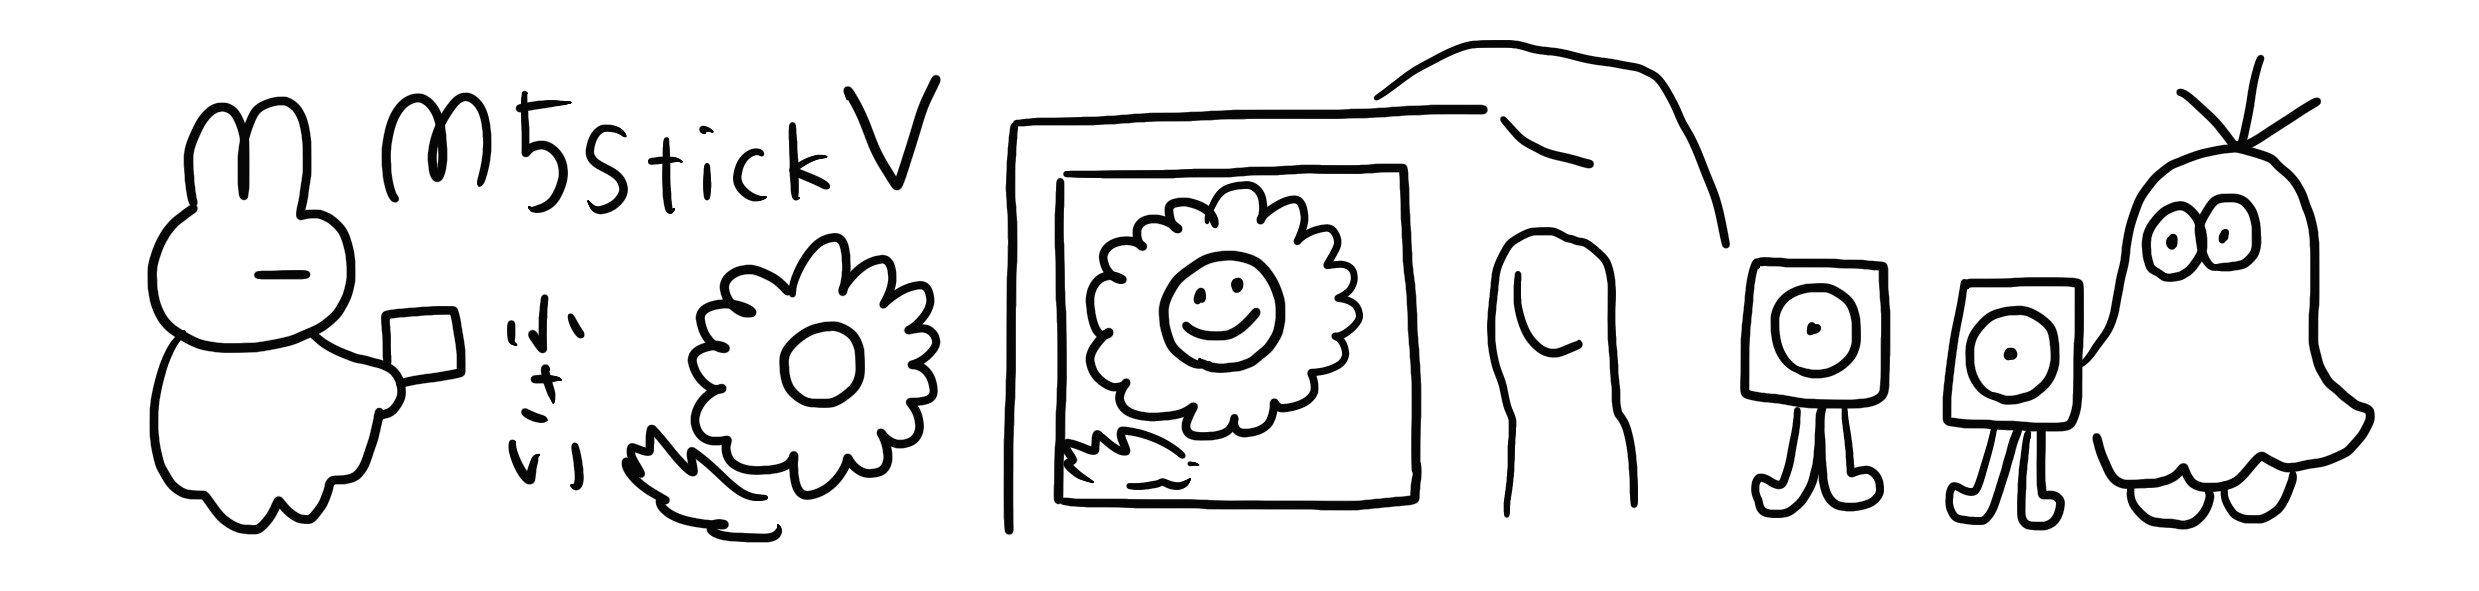
\includegraphics[width=\textwidth]{images/202101/newsletter202102_2.png}


\AddToShipoutPictureBG*{%
  \AtPageLowerLeft{%
    \includegraphics[width=\paperwidth,height=\paperheight]%
      {images/p023-bg.jpg}
  }%
}%

\begin{multicols}{2}
カメラ+スピーカー+モニター+KPUが一口サイズの小さい機械に搭載されたM5StickVという機械があります。KPUが搭載されているので、AIのモデルを入れて顔認識などをさせることが可能です。
このM5StickVを使って冷蔵庫のプリンを食べてしまう犯人を検出しよう! という趣旨で書かれた本です。こういうノリは好きです。書いてある手順通りやっていけばM5StickVでかなり遊べて楽しい本でした。
\end{multicols}


 
\subsubsection*{『Jupyter BookでAIの解説本を書く方法』ZENKEI AI FORUM 中野裕 著}
(\url{https://techbookfest.org/product/5840767786418176})

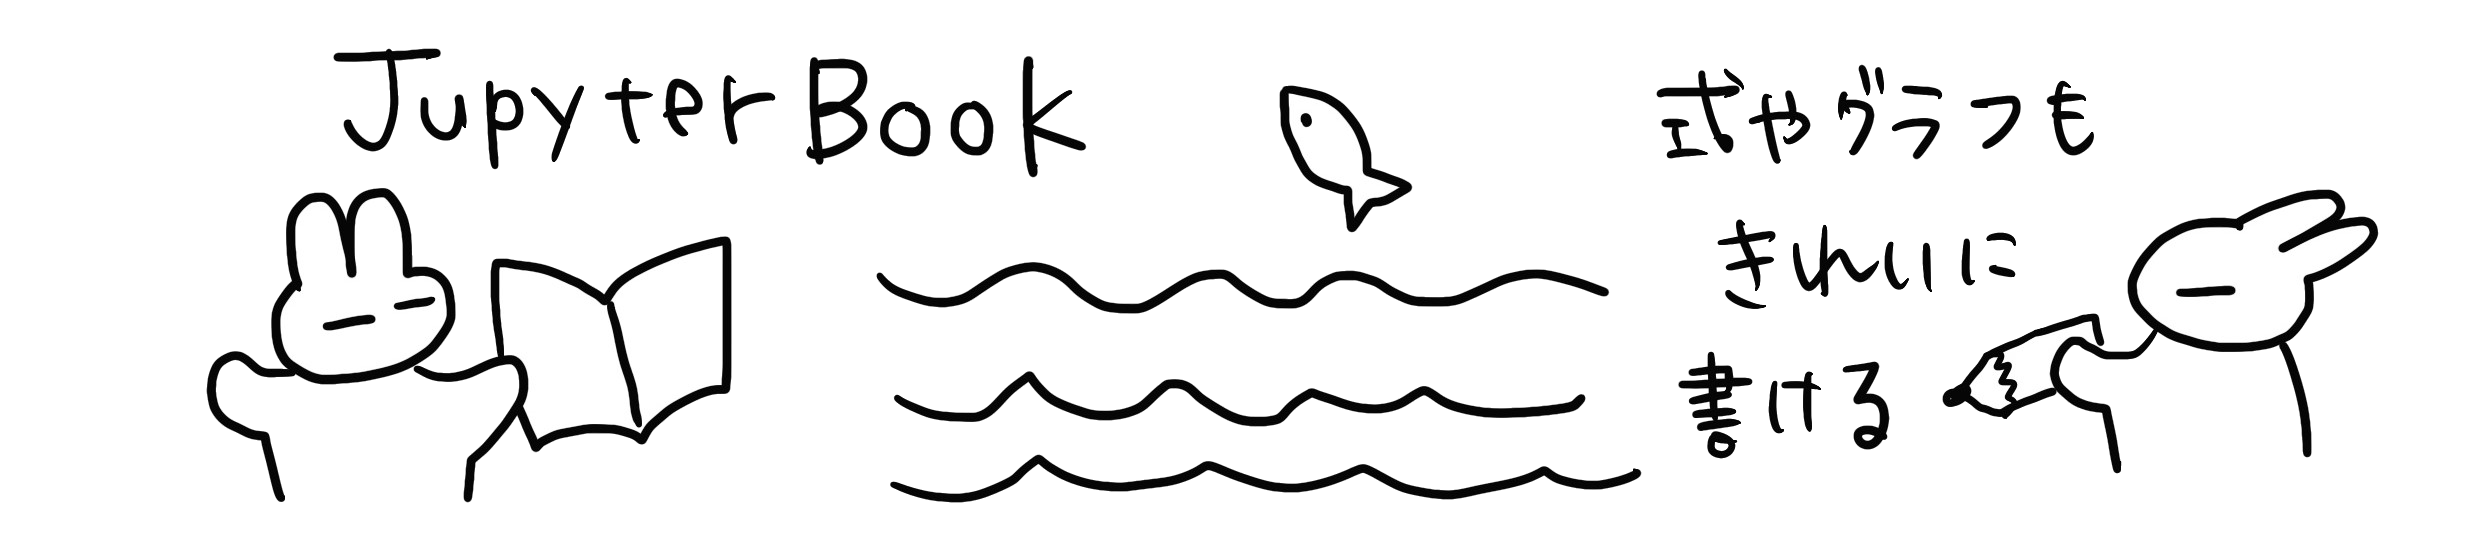
\includegraphics[width=\textwidth]{images/202101/newsletter202102_3.png}


\begin{multicols}{2}
同じZENKEI AI FORUM のかたが書いた本です。

なんとこの本を書きながらJupyterBookについて学ばれたそうで、この本自体がJupyterBookでのサンプルとなっています。

 % 全角空白

 % 全角空白
\end{multicols}


\subsection*{DALL・E}
\addcontentsline{toc}{section}{DALL・E}
(\url{https://openai.com/blog/dall-e/})

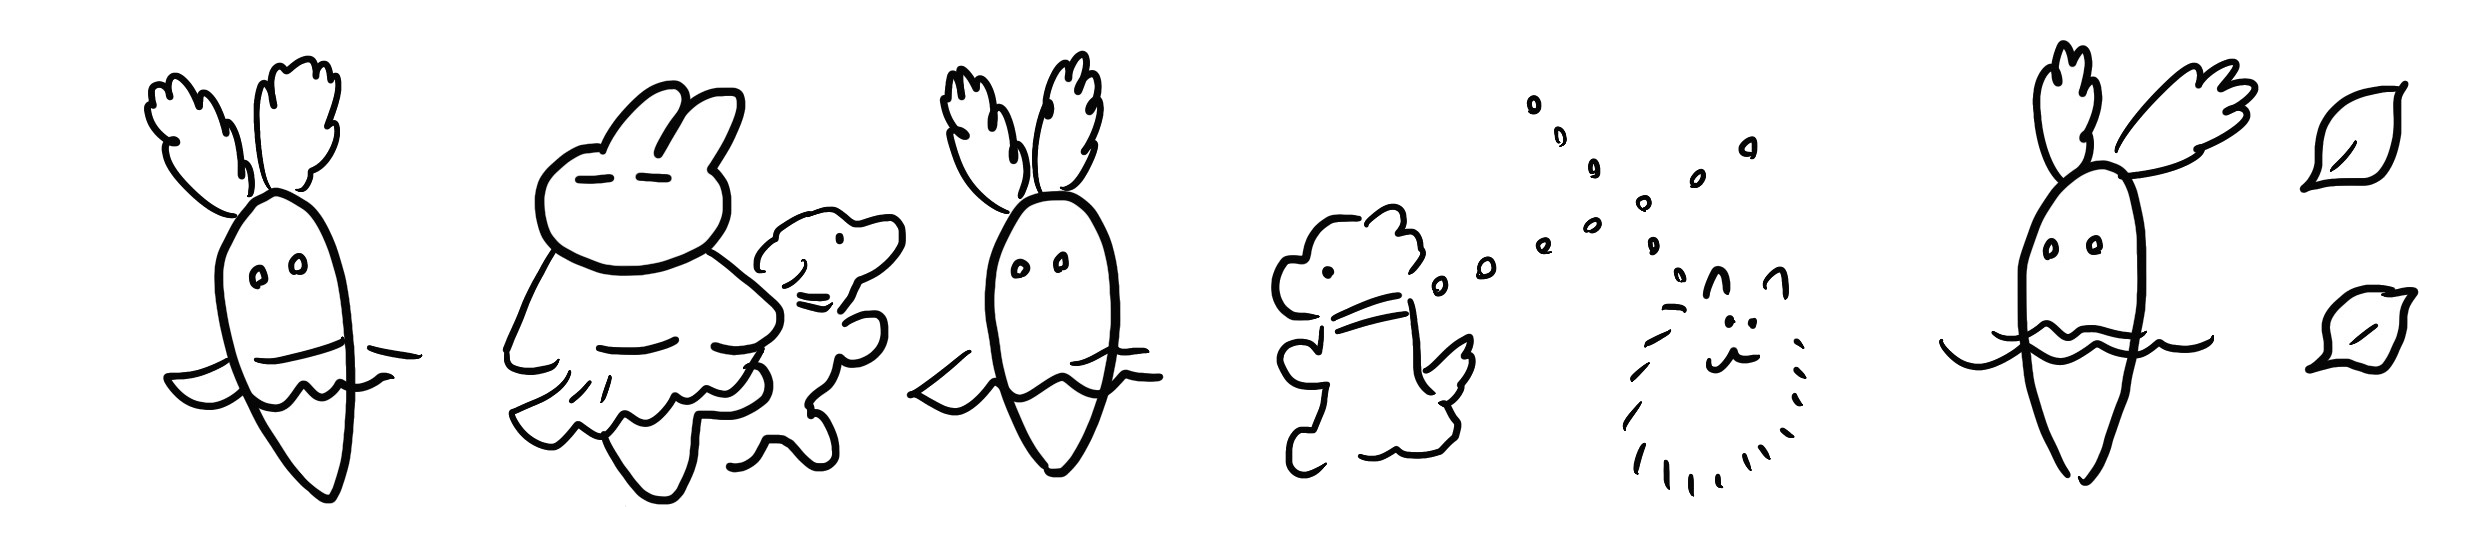
\includegraphics[width=\textwidth]{images/202101/newsletter202102_4.png}
\begin{center}
an illustration of a baby daikon radish in a tutu walking a dog\\
※この記事内の絵はすべて私が描いたものです。DALL・Eの絵は上記リンクよりご確認ください。
\end{center}


\begin{multicols}{2}
OpenAI(人工知能を研究する非営利団体)が発表したAI「DALL・E」について。

\AddToShipoutPictureBG*{%
  \AtPageLowerLeft{%
    \includegraphics[width=\paperwidth,height=\paperheight]%
      {images/p024-bg.jpg}
  }%
}%

DALL・Eは人間が入力した一連の言葉を絵に描いて出力するAIです。例えば「犬の散歩をしているチュチュを着た大根の赤ちゃんのイラスト(an illustration of a baby daikon radish in a tutu walking a dog)」と文章を入力すると、その通りを絵に描いたイラストが出力されるとのことです。“犬”や“大根”など一語から描くだけでもすごいと感じますが、複雑な文章も理解して描けるということです。出力例で見る限りでは、チュチュと大根がばらばらに並んでいたり、犬のほうがチュチュを着てしまったりということがないようなのです。大根の赤ちゃんには、ご丁寧にも赤ちゃんぽいかわいいお顔と犬の散歩のための手足が描かれています。説明によると、手足があって服を着ている大根の絵をあらかじめAIに学習させていたわけではなく、着衣の人間の絵を学習したことで、AIが大根の絵に“着衣”である状態を適用しているそうです。

実際に全文を入力してDALL・Eを試すことはできませんが、上記のURLのページの中ごろに黒枠で囲まれたところがありますので、その黒枠をクリックすると、テキストの一部を変更させた出力結果を見ることができます。

モデルについては、「文章と画像のペアのデータセットを使って、文章から画像を生成するよう訓練された120億パラメータのGPT-3」と説明されています。120億パラメータとはめちゃくちゃ多いですね! 一般のAIユーザにはちょっと手が出ない規模の機器が必要になりそうですが、出てきた絵のすばらしさを見れば納得ではあります。
\end{multicols}


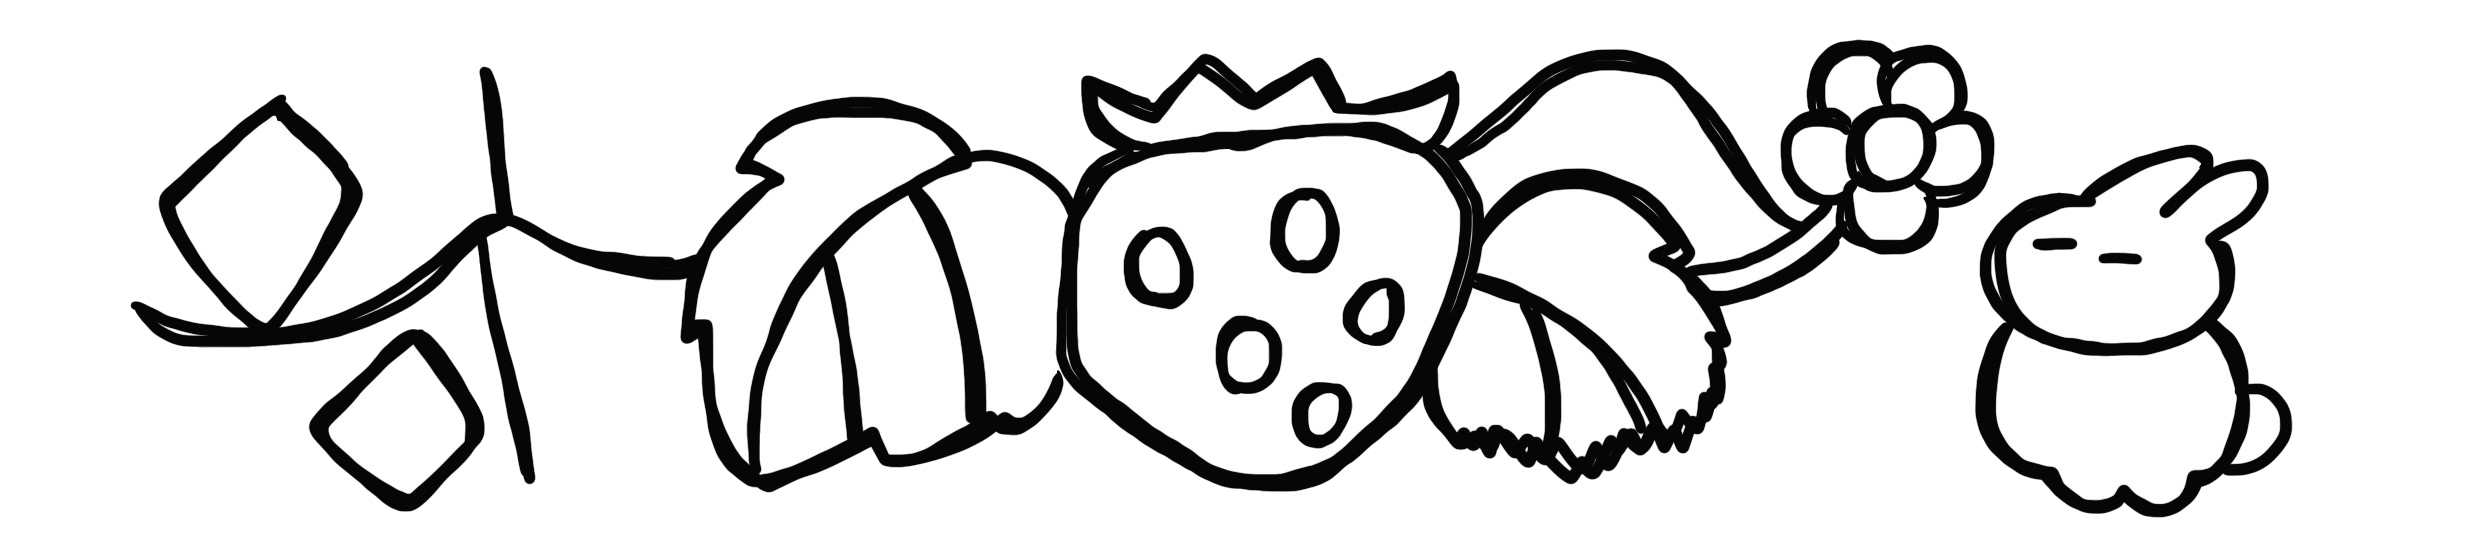
\includegraphics[width=\textwidth]{images/202101/newsletter20210218.png}
\begin{center}
a stained glass window with an image of blue strawberry\\
このテキストでOpenAIが作成した画像はとてもかわいくて好きです。
\end{center}


\begin{multicols}{2}
\subsubsection*{蛇足1}
このパラメータ数を単純に生き物の神経細胞の数と比較するのはあまり意味のない行為ですが、一応調べてみました。wikipediaによると、大脳新皮質の神経細胞の平均数は、成人女性は190億、成人男性は230億、全身では1000億との推計がされています。人間の大脳新皮質の神経細胞の数は、ナガスクジラ(150億:体長20m~)やアフリカゾウ(110億:体長6m)よりも多く、ヒレナガゴンドウ(372億:体長6m、大脳の大きさは人間の2倍)よりも少ないということになります。
\end{multicols}


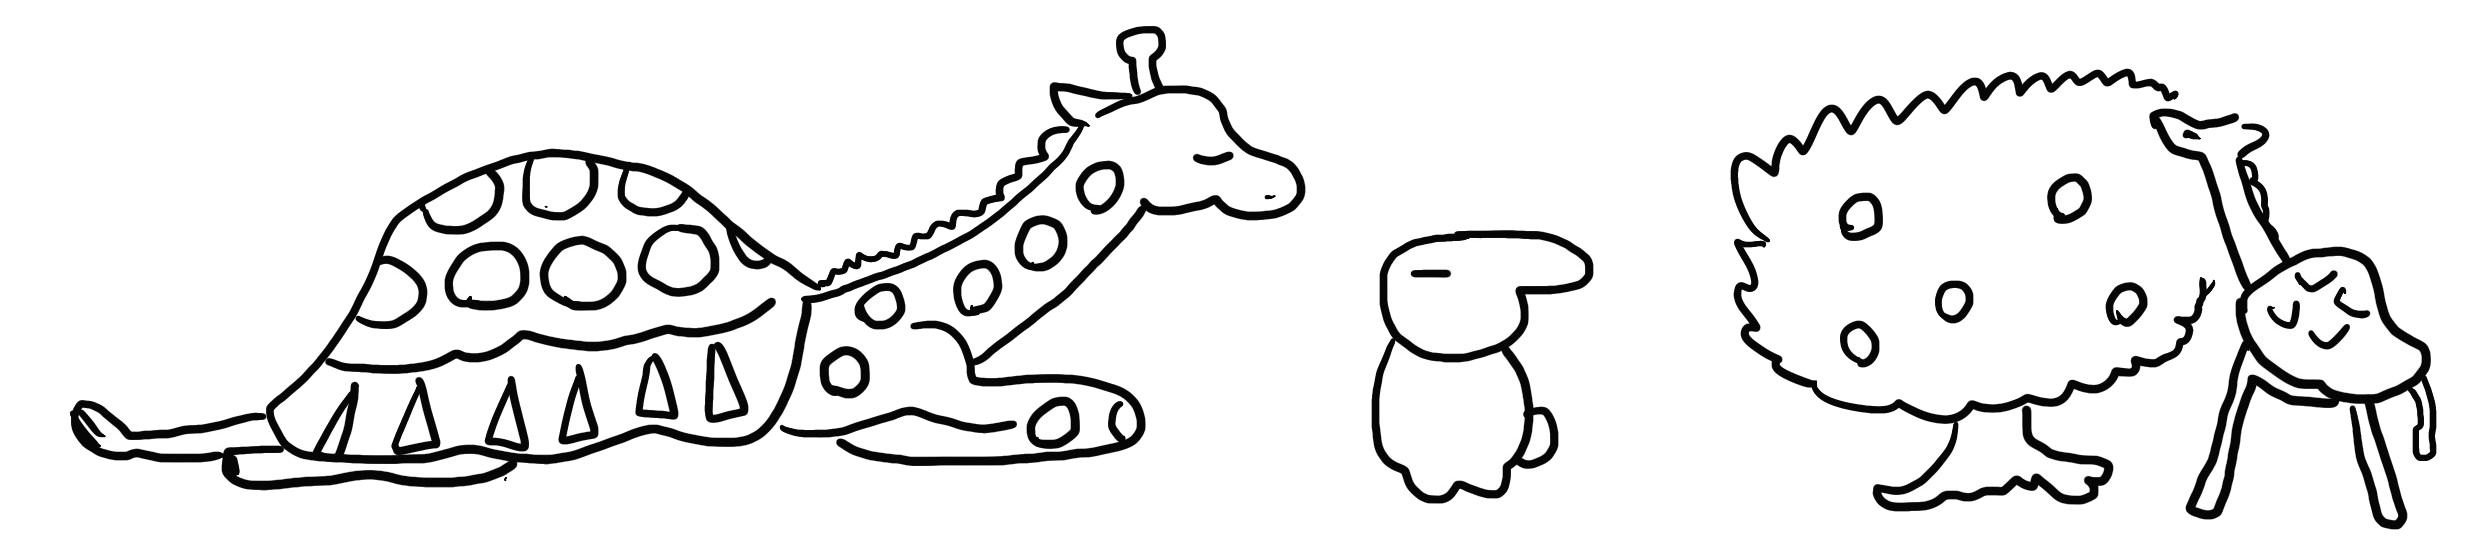
\includegraphics[width=\textwidth]{images/202101/newsletter20210218_1.png}
\begin{center}
  a professional high quality illustration of a giraffe turtle chimera
\end{center}


\begin{multicols}{2}
\subsubsection*{蛇足2}
こうなってくると気になるのがヒレナガゴンドウって何? ということです。ヒレナガゴンドウはイルカの一種で、北大西洋や南極の周りの海に生息しています。社会性が高く、つるんで行動する性質があるようです。おでこにメロンと呼ばれる脂肪体(エコーロケーションに使用すると推測されている)があるのと長い鎌形のヒレが特徴です。100個体ほどの群れを作り、肉食で、シャチにも勝つようです。寿命は、雄が45歳、雌が60歳ほどだそうです。
水中では敵なしで悪天候と人間以外は恐れるものはなく長生きとなると割と人生に余裕がありそうに思うのですが、退屈は感じないんでしょうか。イルカは、本を読まないし絵も描かないしアクセサリーを身に着けたりシールを集めたりもしないですよね。何して遊んでいるんだろう、、ある種のイルカはフグ毒を少量摂取してラリって遊ぶらしいですが、、いやそういう過激なんじゃなくて、、もっとカジュアルなのがないのかな、、いや遊びというもの自体が生存という観点からしたらやらなくていいことをやっているわけでそもそもちょっと危険なものなのか、、
動物ってなんであんなに群れで仲良くできるんだろう、生きていくためにはそうするしかないのかなと思っていました。しかし遊び道具がないならば、友達とだべって歌って踊っているのがいちばん手っ取り早く安全で楽しいのかもしれません。
 

ちなみに“イルカ 何をして遊ぶのか”で検索したら、“コロナ 遊び”と“大人 遊び”が他の検索案として出てきました。コロナは、、時代ですね、えっと、個人的にはこの機会に家事を覚えるのもいいんじゃないかと思います。マスク入れを自分で作ってみるとか。私はそもそもインドア派なのですが、この期間に家でできる遊びのレパートリーがまたふえました。例えばこんな感じです。

\paragraph{\gtfamily\bfseries ■炊飯器クッキング}
炊飯器調理は調理は簡単だけど待ち時間のかかるものが多いですが、在宅勤務であれば無問題です。

\paragraph{\gtfamily\bfseries ■AIクッキング}
料理画像からレシピを生成するというAIモデルが存在しており、InverseCookingという名前で提供されています (\url{https://github.com/facebookresearch/inversecooking})。これを使えば、写真でしか見たことのない料理も自分で作ることができます。ただし、分量は出力されないため、味つけはカンで行う必要があり、料理をある程度知っている人向けと言えます。また、モデルは主に西洋料理を学んでいるようでアジア料理は解釈が間違って変なレシピになってしまうことがあります。そのギャップも楽しむものとして私は利用しています。この但し書きがドラえもんのひみつ道具っぽいですね。
 
\paragraph{\gtfamily\bfseries ■オンラインダンスレッスン受講}
YouTubeやInstagramで無料で配信されているかたもいます。ジャンプしない、集合住宅でもできるプログラムもたくさんあります。
私は正直、とりあえず体を動かせればよくて、これでダンスが踊れるようになるとは思っていなかったです。だって、“どうせオンラインだし” 受講者に合わせて細かいところまで教えられないでしょ。プログラミングならまだ画面を止めてコードを読んだりして各自のスピードで学習できるかもしれないけど、ダンスでは無理じゃない。もともとうまい人じゃないとオンラインでは学べないよね、と。ところが、私が受けているダンスの先生は、同じダンスに対して3種類の動画を出していたんです。音楽つきで通常スピードのもの、先生がゆっくり曲を口ずさみながらスローテンポでちょっと大げさに踊っているもの、一つ一つの動作を解説しているもの、すべて鏡になっていて、先生が動いたほうへ動けばいいようになっています。
先生は動画で「みんながどうやったらオンラインでダンス踊れるようになるか考えてこうしてみたんだけど、もしもっといい方法が見つかればまた変えます」と言っていて、まじめだなと私はおどろきました。そしてファッションがいつもおしゃれで、突然ヒョウ柄で出てきたりしてかわいいんです。“どうせこんなもんでしょ”っていう考え方は本当に間違ってるなあ、、やる人はなんでも工夫してやるもんだ、、と思いました。


\AddToShipoutPictureBG*{%
  \AtPageLowerLeft{%
    \includegraphics[width=\paperwidth,height=\paperheight]%
      {images/p026-bg.jpg}
  }%
}%

“大人 遊び”というのは、一つには、大人になったら友達と遊ぶとしたらお酒を飲みにいくばかりで子どものときみたいに鬼ごっこやトランプで盛り上がったりできない、何かいい遊びはないか、というちょっと切ない検索なのですね。大人だって鬼ごっこしてもいいんですが、このご時世集まれないというのと、そうでなくても仕事終わって夜八時とかに大人が全力で鬼ごっこできる場所ってあまりなさそうですよね。ほか、大人ならではの遊びとして、キャンプなんて素敵ですけど、毎晩は行きづらいですし。
うん、それなら、AIフォーラムに来たらいいじゃない、オンラインだし。というのは冗談として、サークルを作って、あるいは一人ででも、本を一冊書いてみるというのはいかがでしょうか。なんでも自分のしたいように作れますし、できたものを、会ったこともないどこかの誰かが読んでくれるというのは、独特な喜びがあります。

ではまた。電子の海でお会いしましょう。
\end{multicols}


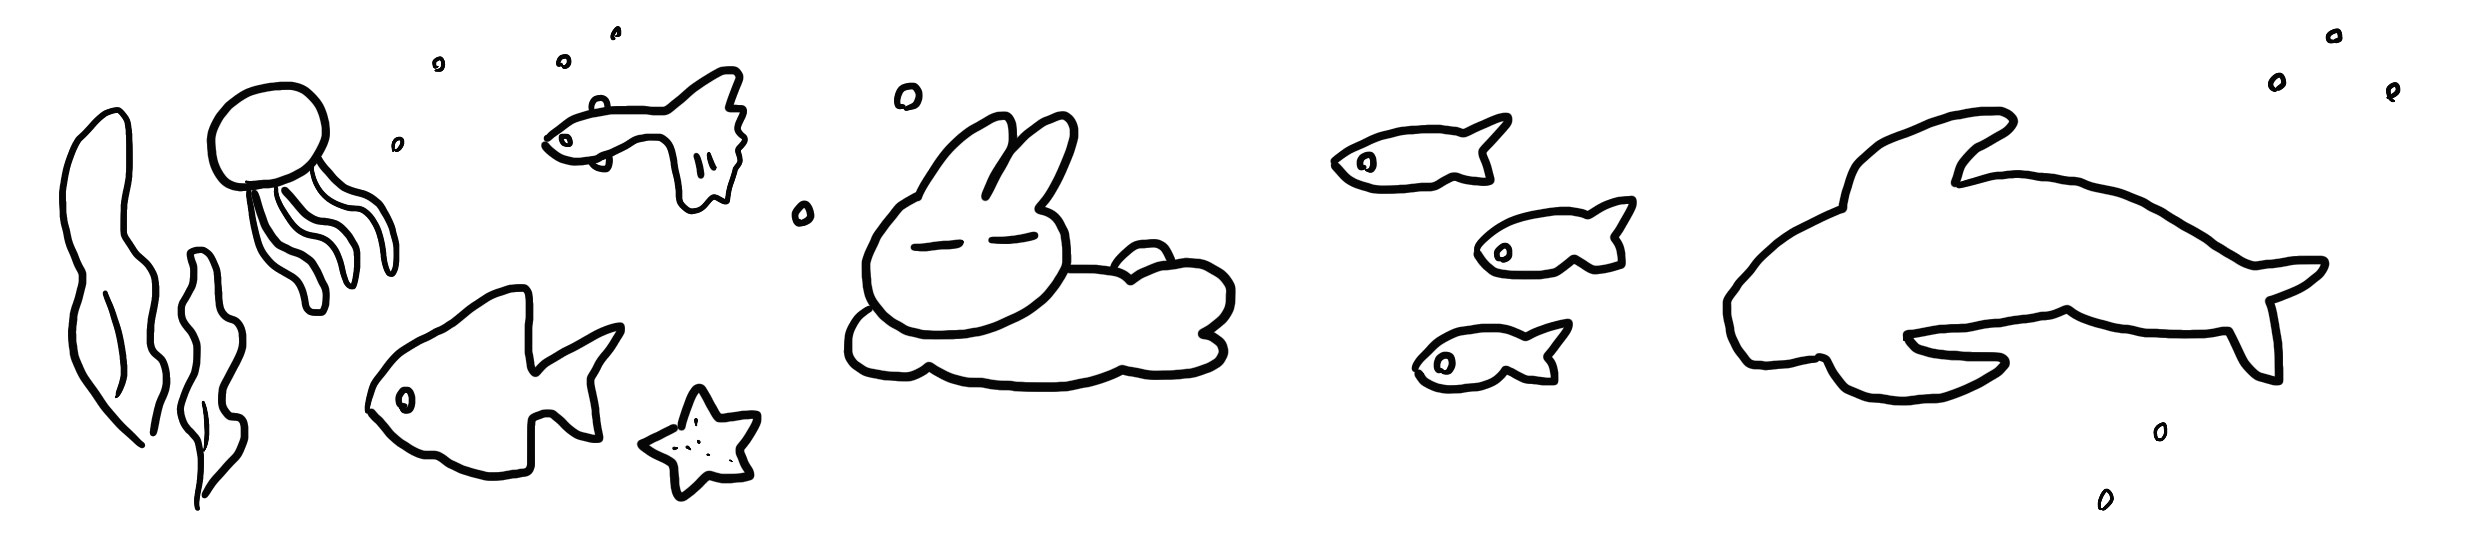
\includegraphics[width=\textwidth]{images/202101/newsletter20210218_3.png}


\newpage

\chapter*{技術書典10に参加して(中野裕)}
\addcontentsline{toc}{chapter}{技術書典10に参加して(中野裕)}
\thispagestyle{fancy}
\AddToShipoutPictureBG*{%
  \AtPageLowerLeft{%
    \includegraphics[width=\paperwidth,height=\paperheight]%
      {images/p027-bg.jpg}
  }%
}%


\textit{〜 「Jupyter BookでAIの解説本を書く方法」の著者への妄想インタビュー 〜}

\vspace{1em}

これから記載するインタビュアーと著者との会話は、著者自身がインタビューを受けたことを妄想しながら頭の中で行った仮想のインタビューです。なお、著者の回答として記載した内容は妄想ではなく真実です。

\vspace{0.45cm}

\begin{multicols}{2}

\paragraph{\gtfamily\bfseries 【司会】}
\textbf{それでは、「Jupyter BookでAIの解説本を書く方法」の著者である中野 裕さんに執筆期間のお話を伺っていきたいと思います。よろしくお願いします。}

\begin{quotation}
  \noindent (筆者)
よろしくお願いします。
\end{quotation}


\noindent
\textbf{まず、今回の技術書典10で本を書こうと思ったきっかけなどはありましたか。}


\begin{quotation}
  \noindent
たしか9月のZENKEI AI FORUMだったと思います。その回は市來さんと古川さんが技術書典9での体験談をお話されていました。その中でJupyter Bookの話題が出たのですが、本当に軽い気持ちで「使ってみたいな」とYouTubeのライブ配信側のチャットでコメントしたところ、そのあとすぐに市來さんから本を書いてみましょう!とお誘いいただきました。一瞬「あ、しまっ・・」と思いましたが、最近ZENKEI AI FORUMでも特に発表者として参加できていなかったので、いい機会だなと思い直し、やってみようと決めました。
\end{quotation}

\noindent
\textbf{なるほど、流れに流されてみるのもいいものですよね。技術書典10は12月下旬から1月上旬でしたが、いつ頃から作業を開始したのですか。}

\begin{quotation}
  \noindent
やると決めたすぐ後から着手しました。個人的なことですが、子供が生まれたばかりで、仕事以外のほとんど時間が育児という毎日でしたので、少しずつでも書いていかないと間に合わないという思いがありました。寝る前の1時間や朝活として1時間早く起きてやったり。朝活は見事に三日坊主でしたが・・・。私はどちらかというと夏休みの宿題をギリギリまで取っておくタイプでしたので、約3ヶ月間少しずつでもコンスタントに作業できたことは自分でも驚いています。
\end{quotation}


\noindent
\textbf{最初から書く内容は固まっていましたか。}


\begin{quotation}
  \noindent
いいえ、ゴールは全く見えていませんでした。なんといってもJupyter Book自体使ったことがなかったので。とりあえず、Jupyter Bookの公式サイトを読み込むことから始めました。本の中でも何度か触れていますが、Jupyter BookはWEBコンテンツとしての機能が豊富で、アウトプットとしてはHTML形式が適していたのですが、技術書典の出展の形式がPDFやEPUBといったものだったので、Jupyter Bookからの出力としてPDFを採用すべきか悩みました。結果的にはPDF形式で出力し、どの程度書籍としての表現ができるかを試してみようと思いました。
\end{quotation}


\noindent
\textbf{本のタイトルは「Jupyter BookでAIの解説本を書く方法」ですが、それはどのように決まったのですか。}


\AddToShipoutPictureBG*{%
  \AtPageLowerLeft{%
    \includegraphics[width=\paperwidth,height=\paperheight]%
      {images/p028-bg.jpg}
  }%
}%

\begin{quotation}
  \noindent
Jupyter BookはAIのためのツールではありません。ただ、Jupyter BookはJupyter notebookをページの素材として扱うことができ、Jupyter notebookは今までのAIの勉強で溜まったものがあったので、そのAIの勉強用に作成したnotebookを活用してJupyter Bookで本のようなクオリティの出力に仕上げようと思いました。サークルもZENKEI AI FORUMだったので、AIの内容を入れたかったところもあります。内容がタイトルに負けていないかなと度々心配になりました・・・。
\end{quotation}


\noindent
\textbf{この本でAIを解説するのではなく、AIを題材とした本を書くためのツールとしてJupyter Bookを紹介しているということですね。}


\begin{quotation}
  \noindent
はい、そうです。
\end{quotation}


\noindent
\textbf{今回、本書を価格500円で販売されていましたが、価格の決め方みたいなものはありましたか。}


\begin{quotation}
  \noindent
書き始めた頃は無料で配布しようと思っていました。有料にする場合の最低価格は500円と決まっていて、500円の価値があるかと考えた時に自信がなかったこともあります。しかし、考えようによっては最近のちょっとしたデザートでも500円くらいしますし、執筆に費やした時間もそれなりにかかったので、価格設定として500円は妥当かとも思うようになりました。最終的には市來さんに背中を押していただき、有料500円と決めました。実際、イベント開催中に購入されましたと聞くたびに、購入者の期待に答えられているだろうかという不安が増大していきました。有料にしたことによってページ数も気になり、フォントサイズを大きくしてページ数を増やしたりもしました。Jupyter BookからPDFで出力すると書籍としては文字が小さいので、フォントサイズを大きくすることで「本らしさ」が出たようにも思います。最終的に43ページになりました。
\end{quotation}


\noindent
\textbf{価格の設定は難しいですよね。ただ、有料にすることで得られた経験もあったということですね。}


\begin{quotation}
  \noindent
何事も経験ですかね。
\end{quotation}


\noindent
\textbf{今回、このJupyter Bookを題材とした本を書くに当たって、自分の中であるルールを定めていたと聞きましたが。}


\begin{quotation}
  \noindent
はい。当然と思われるかもしれませんが、本のネタを集めるにあたり、Jupyter Bookとその周辺の必要な技術の情報源としてはそれぞれの公式サイト以外は見ないというルールを自分に課しました。
\end{quotation}


\noindent
\textbf{それはどのような意図があったのでしょう。}


\begin{quotation}
  \noindent
私の本業はシステムエンジニアですが、技術的な情報を得る方法としてよくQiitaなどの技術紹介のサイトを見ます。知りたいと思ったことが見つからないことがないくらい、必ず誰かが技術を紹介してくれています。今回のJupyter Bookに関しても探せば面白い情報が見つかるとは思いますが、本を書くことは自分が情報の発信者になるということですので、自分の言葉だけで書き上げなければという思いがありました。
\end{quotation}


\noindent
\textbf{では、本の内容について紹介をお願いできますか。}


\begin{quotation}
  \noindent
本書はPythonで書かれた一つのDeep Learningのプログラムコードから始まります。CIFAR-10の画像分類をKerasを使って実装した短くてとてもシンプルなコードです。実際に動かして結果を得るだけであればこのプログラムで十分ですが、プログラムの解説を行ったり、学生や研究者の論文、会社では成果報告などプログラムだけでは十分ではなく説明を加える必要があるでしょう。そのような場面を想定して、純粋なプログラムをドキュメント(読み物)に変化させていきます。ドキュメントの品質を向上させるためのツールとして、Jupyter notebook、markdown、そしてJupyter Bookを紹介しています。
それらのツールを使うためには、様々なソフトウェアのインストールやライブラリの取得が必要ですが、本書を読んで試してみようとする方が環境構築で躓いてやる気をなくしてしまうことがないように、丁寧に書くように心がけました。
その純粋なDeep Learningのプログラムに説明文や数式、グラフを付けていきますが、「こういう風に説明を書いていくんだよ」という飾りの説明文ではなく、ZENKEI AI FORUMらしくAIのプログラム自体に関しても理解してもらえるように正確に書きました。そして、最後の章では見た目をよくするためにJupyter Bookの活用の仕方を紹介しているといった流れになります。
\end{quotation}


\AddToShipoutPictureBG*{%
  \AtPageLowerLeft{%
    \includegraphics[width=\paperwidth,height=\paperheight]%
      {images/p029-bg.jpg}
  }%
}%

\noindent
\textbf{いろんな要素が詰まった本だったんですね。}


\begin{quotation}
  \noindent
一つのテーマで仕上げるには知識が足りなかったというだけかもしれません。私の今までの経験をパッチワークのように繋ぎ合わせてようやくそれなりのボリュームが出せたというのが正直なところです。
\end{quotation}


\noindent
\textbf{実際にJupyter Bookを使ってみて率直にどうでしたか。}


\begin{quotation}
  \noindent
普段Jupyter notebookで研究結果や調査結果をまとめている人にとっては、それらをWEBページとして公開する目的においては非常に便利で簡単なツールだと思います。自動的に目次(ナビゲーション)も付けてくれますし、Jupyter notebookの実行結果としての画像やグラフもWEBページ上にそのまま表示させることができます。さらに、そのWEBページ内にインタラクティブな要素も持たせることができるので、表現の幅もJuypter notebookより広がります。
一方で、今回のPDF形式での出力においてはWEBページで効果的なインタラクティブな効果をつけることができないこともあり、Jupyter Bookの良さを十分に発揮させることができないと感じました。
\end{quotation}


\noindent
\textbf{では、Jupyter BookでのPDF形式での出力を上手に仕上げることが本のテーマだったと思いますが、内容をまとめるのに苦労されたということでしょうか。}


\begin{quotation}
  \noindent
そうですね、苦労は多かったと思います。まず、最初にPDF形式で出力させてみたところ、日本語が中華フォントになってしまいPDFでの出力を諦めかけました。結果的には、Jupyter Bookのバージョンが上がったのかこの問題はいつの間にか解決していました。
次に、WEBページでは目次(ナビゲーション)はとても便利でしたが、PDFでは機能しないため取り除きたかったのですが、取り除くための方法がなかなか見つかりませんでした。一時はPDFを直接編集して取り除けないかということも考えましたが、Jupyter Bookの仕組み(CSSを追加する方法)で取り除くことができることがわかりました。この辺りで徐々にPDF形式でいけるというイメージを持ち始めてきました。
最後に、取り除いた目次部分がページの余白として不自然に残ってしまっていてバランスの悪いレイアウトになっていましたが、その余白を注釈用のスペースとして活用することで、全体的なバランスがよくなりました。この注釈をつける機能もJupyter Bookから提供されているもので、PDF形式での出力結果に「本らしさ」を加えてくれます。
このように試行錯誤を繰り返し、さらに運にも恵まれて完成まで持っていくことができました。
\end{quotation}


\AddToShipoutPictureBG*{%
  \AtPageLowerLeft{%
    \includegraphics[width=\paperwidth,height=\paperheight]%
      {images/p030-bg.jpg}
  }%
}%

\noindent
\textbf{Jupyter Bookでオススメの機能はありますか。}


\begin{quotation}
  \noindent
やはり「タグ」の機能ですね。タグはJupyter notebookのコードセル(Pythonでプログラムを書く部分)の実行結果をJupyter Bookの出力としてどう表現するかを指示するものです。例えば、Jupyter notebookでプログラムの実行結果をグラフとして出力する場合、matplotllibを使ってグラフ描画用のプログラムをコードセルに記載します。ただ、このプログラムはユーザにグラフを見せるためのものであって、プログラムそのものをユーザに見せる必要はありません。グラフだけ見えればいいのです。こういった時に、プログラムの実行結果(グラフなど)だけを表示させて、プログラム部分は見せないということがタグという機能で実現できます。
\end{quotation}


\noindent
\textbf{なるほど、Jupyter notebookに記載された内容を全てBookとして表示するのではなく、必要な部分だけを表示するように制御できるということですね。}

\begin{quotation}
  \noindent
はい。技術的なことではありませんが、もう一つ面白かったことがあります。Jupyter Bookは現時点ではβ版であり今後も改良されることが期待されますが、改良のリクエストをユーザから募り、他のユーザからも同意を得られたものがランクアップしていく仕組みが興味深かったです。予め投稿されていた要望に共感するものがあれば「いいね」と同意すれば要望が製品に反映される可能性が高まります。また、他のユーザの要望を見ることで、自分以外のユーザがどういうことを気にしているかがわかります。①多くのユーザの声を集めることができる ②ユーザ自身が要望を分類してくれる ③ユーザ同士の情報共有の場にもなる。シンプルだけどメリットがたくさんある良い仕組みだと思いました。
\end{quotation}



\noindent
\textbf{ツール自体だけでなく、その開発プロセスにも面白さがあったということですね。それでは最後に今後の活動について聞かせていただけますか。}


\begin{quotation}
  \noindent
技術書典10ではPDFのみの販売としましたが、もう少しレイアウトに「本らしさ」を加えられたら物理本として出してみたいです。ただし、Jupyter Bookの機能によって実現すべきことですので、今後のJupyter Bookの改良にも注目していきたいと思います。
\end{quotation}

\end{multicols}

\newpage

\chapter*{著者紹介}
\addcontentsline{toc}{chapter}{著者紹介}

\AddToShipoutPictureBG*{%
  \AtPageLowerLeft{%
    \includegraphics[width=\paperwidth,height=\paperheight]%
      {images/ZAM202101-authors-bg.png}
  }%
}%

\noindent
{\gtfamily\bfseries \Large 第1章、第2章}

\noindent
{\large \ruby{市來}{いちき}\ruby{健吾}{けんご}}

金沢の全景株式会社でプログラマをやっています。
またその活動の一つとして 2017 年から「ZENKEI AI FORUM」という
地域コミュニティの運営もやっています。

ぼくは 2009 年に日本に帰国するまでは物理の研究者として
大学や研究所で研究をしていました。
これまで住んできた街は、広島、仙台、京都、パサデナ(アメリカ)、
エンスヘデ(オランダ)、ボルチモア(アメリカ)、ロンドン(カナダ)、
エドモントン(カナダ)、金沢です。

\vspace{1em}

\noindent
{\gtfamily\bfseries \Large 第3章}

\noindent
{\large furukawa}

石川県金沢市を拠点としている「ZENKEI AI FORUM」というAI活用のサークルで
『ゼロからはじめるAI』と題して、画像分類やGANについてなどの話をしたりしています。


\vspace{1em}

\noindent
{\gtfamily\bfseries \Large 第4章}

\noindent
{\large \ruby{中野}{なかの}\ruby{裕}{ゆたか}}

1979年石川県白山市(旧 松任市)生まれ。
金沢大学大学院自然科学研究科数物科学専攻修士課程終了。
東京でシステムエンジニアとして約13年、
組み込み系システム開発や携帯端末(ガラケー)、スマートフォン開発に従事。
現在は石川県にUターンで帰省し、
株式会社シーピーユーで同じくシステムエンジニアとして
CADアプリケーション、スマートフォンアプリ、VRの開発を担当している。


\newpage

\vspace*{\fill}

% 奥付
\begin{flushleft}
  \begin{tabular*}{\textwidth}{@{}l@{\extracolsep{\fill}}}
    \textbf{\LARGE 月刊 ZENKEI AI MAGAZINE}\\
    \textbf{\Large 2021年1月号}\\
    \bhline{1pt}
    \begin{tabular}{@{}r@{年\kern.5zw}r@{月\kern.5zw}r@{日\kern1.5zw}ll}
      2021 & 2 & 24 & 初版発行 & (オンライン)\\
      2021 & 3 & 31 & 改訂版発行 & (第1刷)\\
      2021 & 7 & 26 & 第3版発行 & (オンライン)\\
    \end{tabular} \\
    \\
    \begin{tabular}{@{}l@{\kern.5zw\textbf{:}\kern1zw}l}
      \textbf{編 集} & ZAM 編集部\\
      \textbf{発行者} & 市來健吾\\
      \textbf{発行所} & ZENKEI AI FORUM\\
      \textbf{連絡先} & \url{https://forum.ai.zenkei.com/}, \href{https://twitter.com/zenkeiaif}{@zenkeiaif} \\
      \textbf{表 紙} & 市來健吾\\
      %\textbf{印刷所} & ちょ古っ都製本工房 \url{https://www.chokotto.jp/} \\
    \end{tabular} \\
    \bhline{1pt}
    \texttt{%
      \textcopyright\quad
      ZENKEI AI FORUM\quad
      2021,\quad
      Printed in Japan
    }
  \end{tabular*}
\end{flushleft}


\newpage

\AddToShipoutPictureBG*{%
  \AtPageLowerLeft{%
    \includegraphics[width=\paperwidth,height=\paperheight]%
      {images/ZAM202101-backcover-v2.jpg}
  }%
}%

 % 全角空白

\end{document}
